\documentclass{report}

\usepackage{amsmath,
            amssymb,
            amsthm,
            atbegshi,
            caption,
            epigraph,
            etoolbox,
            enumitem,
            fancyhdr,
            geometry,
            graphicx,
            hyperref,
            kpfonts,
            lipsum,
            longtable,
            minted,
            thmtools,
            tikz, tikzpagenodes,
            titletoc,titlesec,
            tocloft,
            wrapfig}
\usetikzlibrary{positioning}
\definecolor{darkred}{cmyk}{0.0,0.87,0.87,0.50}
\colorlet{mygray}{black!20}

\renewcommand*\rmdefault{iwona}


\setlength\epigraphwidth{15cm}
\setlength\epigraphrule{0pt} % line between quote and quoter
\makeatletter
\patchcmd{\epigraph}{\@epitext{#1}}{\itshape\@epitext{#1}\/}{}{} % italics 
\makeatother

% To sort the definitions:
% awk '/^\\begin\{(definition|theorem|proof)\}/,/^\\end{(definition|theorem|proof)}/ { printf "%s\0",$0} /^\\end{definition}/ { print ""}  END {print ""}' PENSUM.tex | sort -t'\0' | tr '\0 ' '\n' 

% \pagestyle{fancy}
\pagenumbering{Roman}
\setcounter{tocdepth}{1}
\graphicspath{{src/fig/}}

\newtheoremstyle{definitionstyle} % name
    {\topsep}                    % Space above
    {\topsep}                    % Space below
    {}                   % Body font
    {}                           % Indent amount
    {\sffamily}                   % Theorem head font
    {.\newline}                          % Punctuation after theorem head
    {.5em}                       % Space after theorem head
    {\thmname{#1}\textbf{\thmnote{ #3}}}  % Theorem head spec (can be left empty, meaning ‘normal’)


\newtheorem{theorem}{Theorem}
\theoremstyle{definitionstyle}
% \theoremstyle{nopar}
% \newtheorem{lemma}[theorem]{Lemma}
% \newtheorem*{definition}{\textgreater{}\textgreater{}}
\newtheorem*{definition}{$\rightarrow$}
% \newtheorem{prop}[theorem]{Proposition}

\titleformat{\subsubsection}[runin]% runin puts it in the same paragraph
       {\normalfont\bfseries}% formatting commands to apply to the whole heading
       {\thesubsubsection}% the label and number
       {0.5em}% space between label/number and subsection title
       {}% formatting commands applied just to subsection title
       []% punctuation or other commands following subsection title
\author{Anders Sildnes\\
    NTNU}
\date{\today}

\renewcommand\epigraphflush{flushright}
\renewcommand\epigraphsize{\normalsize}
\setlength\epigraphwidth{0.7\textwidth}

\definecolor{titlepagecolor}{cmyk}{1,.60,0,.40}

\DeclareFixedFont{\titlefont}{T1}{ppl}{b}{it}{0.5in}

\makeatletter                       
\def\printauthor{%                  
    {\large \@author}}              
\makeatother
\author{%
    Anders Sildnes \\
    \texttt{andsild@gmail.com}\vspace{20pt} \\
}

% \definecolor{mygreen}{RGB}{25,170,75}
\definecolor{mygreen}{RGB}{133,149,192}
\definecolor{doc}{RGB}{0,60,110}
\newcommand\Header{%

\begin{tikzpicture}[remember picture,overlay]
\fill[mygreen]
  (current page.north west) -- (current page.north east) --
  ([yshift=50pt]current page.north east|-current page text area.north east) --
  ([yshift=50pt,xshift=-3cm]current page.north|-current page text area.north) --
  ([yshift=10pt,xshift=-5cm]current page.north|-current page text area.north) --
  ([yshift=10pt]current page.north west|-current page text area.north west) -- cycle;
\node[font=\sffamily\bfseries\color{white},anchor=east,
  xshift=-3.2cm,yshift=-1.0cm] at (current page.north east)
  {\fontsize{30}{60}\selectfont Notes and definitions};
\end{tikzpicture}%
}
\newcommand\Footer{%
\begin{tikzpicture}[remember picture,overlay]
\fill[mygreen]
  (current page.south west) -- (current page.south east) --
  ([yshift=-40pt]current page.south east|-current page text area.south east) --
  ([yshift=-40pt,xshift=-3cm]current page.south|-current page text area.south) --
  ([xshift=-5cm,yshift=-10pt]current page.south|-current page text area.south) --
  ([yshift=-10pt]current page.south west|-current page text area.south west) -- cycle;
\node[yshift=0.75cm,font=\ttfamily\bfseries\color{white}] at (current page.south) {\fontsize{20}{24}\selectfont www.stackexchange.com};
\end{tikzpicture}%
}


% \titlecontents{chapter}[0pc]
% {\addvspace{20pt}%
% \begin{tikzpicture}[remember picture, overlay]%
% \draw[fill=doc!30,draw=doc!30] (-3,-.1) rectangle (-.5,.5);%
% \pgftext[left,x=-2.9cm,y=0.2cm]{\color{white}\Large\sc\bfseries chapter\ \thecontentslabel};%
% \end{tikzpicture}
% \color{doc!40}\large\sc\bfseries}%
% {}
% {}
% \;\titlerule\;\large\sc\bfseries Page \thecontentspage%
% \begin{tikzpicture}[remember picture, overlay]
% \draw[fill=doc!25,draw=doc!20] (2pt,0) rectangle (6,0.1pt);
% \end{tikzpicture} % had braces here
% \titlecontents{section}[2.4pc]
% {\addvspace{1pt}}
% {\contentslabel[\thecontentslabel]{2.4pc}}
% {}
% {\hfill\small \thecontentspage}
% []
% \titlecontents*{subsection}[4pc]
% {\addvspace{-1pt}\small}
% {}
% {}
% {\ --- \small\thecontentspage}
% [ \textbullet\ ][]
%
% \makeatletter
% % \chapter*{%
% \renewcommand{\tableofcontents}{%
% \vspace*{-20\p@}%
% \begin{tikzpicture}[remember picture, overlay]%
% \pgftext[right,x=05cm,y=0.2cm]{\color{doc!30}\Huge\sc\bfseries \contentsname};%
% \draw[fill=doc!30,draw=doc!30] (13,-.75) rectangle (20,1);%
% \clip (13,-.75) rectangle (20,1);
% \pgftext[right,x=15cm,y=0.2cm]{\color{white}\Huge\sc\bfseries \contentsname};%
% \end{tikzpicture}%
% \@starttoc{toc}}
% \makeatother
%
% \makeatletter
% \renewcommand{\listoffigures}{%
% \captionof*{aaa}
% \vspace*{-20\p@}%
% \begin{tikzpicture}[remember picture, overlay]%
% \pgftext[right,x=05cm,y=0.2cm]{\color{doc!30}\Huge\sc\bfseries \contentsname};%
% \draw[fill=doc!30,draw=doc!30] (13,-.75) rectangle (20,1);%
% \clip (13,-.75) rectangle (20,1);
% \pgftext[right,x=15cm,y=0.2cm]{\color{white}\Huge\sc\bfseries \contentsname};%
% \end{tikzpicture}%
% \@starttoc{toc}}
% \makeatother







% \pagestyle{empty}
\AtBeginShipoutFirst{\Header\Footer}
\AtBeginShipoutFirst{\Header\Footer}

\newcommand\titlepagedecoration{%
\begin{tikzpicture}[remember picture,overlay,shorten >= -10pt]

\coordinate (aux1) at ([yshift=-45pt]current page.north east); % top right
\coordinate (aux2) at ([yshift=-410pt]current page.north east);
\coordinate (aux3) at ([xshift=-3.5cm, yshift=-55pt]current page.north east);
\coordinate (aux4) at ([yshift=-150pt]current page.north east);

\begin{scope}[titlepagecolor!40,line width=12pt,rounded corners=12pt]
\draw
(aux1) -- coordinate (a)
++(225:5) --
++(-45:5.1) coordinate (b);
\draw[shorten <= -10pt]
(aux3) --
(a) --
(aux1);
\draw[opacity=0.6,titlepagecolor,shorten <= -10pt]
(b) --
++(225:2.2) --
++(-45:2.2);
\end{scope}
\draw[titlepagecolor,line width=8pt,rounded corners=8pt,shorten <= -10pt]
(aux4) --
++(225:0.8) --
++(-45:0.8);
\begin{scope}[titlepagecolor!70,line width=6pt,rounded corners=8pt]
\draw[shorten <= -10pt]
(aux2) --
++(225:3) coordinate[pos=0.45] (c) --
++(-45:3.1);
\draw
(aux2) --
(c) --
++(135:2.5) --
++(45:2.5) --
++(-45:2.5) coordinate[pos=0.3] (d);
\draw
(d) -- +(45:1);
\end{scope}
\end{tikzpicture}%
}

% \include{Style}

\begin{document}
\begin{titlepage}

\noindent
% \titlefont Notes and definitions \par
\par


\epigraph{When we are tired, we are attacked 
by ideas we conquered long ago.}
    {\textsc{Friedrich nietzsche}}
\epigraph{ A musician wakes from a terrible nightmare. In his dream he finds
himself in a society where music education has been made mandatory.}
    {\textsc{Paul Lockhart}}

\null\vfill
\vspace*{1cm}
\noindent
\hfill
\begin{minipage}{0.35\linewidth}
    \begin{flushright}
        \printauthor%
    \end{flushright}
\end{minipage}
%
\begin{minipage}{0.02\linewidth}
    \rule{1pt}{125pt}
\end{minipage}
\titlepagedecoration%
\end{titlepage}

    \begin{abstract}
     An overview of algorithms, words and definitions from my studies as a 
     computer scientist BSc, with an interest in algorithms.

    Note that this document is not intended to be a \textit{public friendly}
    document; it is written by one author and for one author, only. But you
    are still free to read.

    \huge{No guarantee is given to the correctness of the content}
    \end{abstract}
\AtBeginShipoutFirst{\Header\Footer}
\AtBeginShipoutFirst{\Header\Footer}

\tableofcontents
\listoffigures
\listoftables
\pagebreak
% \newgeometry{left=30mm}

\newgeometry{hmargin=2cm,bmargin=3cm,tmargin=4.5cm,centering}
\chapter{Words and Definitions}
\section{Algorithms}\label{section:word}

\begin{definition}[Approximation algorithm]
    Find approximate solutions to~\nameref{optproblem}
\end{definition}

\begin{definition}[Asymptotic Polynomial-time Approximation Scheme, APTAS]
\label{APTAS}
    A family of algorithms, and a constant $c$ such that all solutions has an
    approximation of $(1 + \epsilon)\times{OPT} + c$ for minimization problems.
\end{definition}


\begin{definition}[Bin-packing]
    A series of algorithms to learn how to distribute $n$ numbers into $k$ bins.
    First-fit, best-fit, worst-fit (stack into where there is most free space),
    best-fit, etc.
\end{definition}

\begin{definition}[Complimentary slackness]
    Given an optimal solution to a linear program,
    $Z_{LP}$ and it's dual $Y_{LP}$, with $x_{1}, x_{2}, \dots x_{n}$ and
    $y_{1}, y_{2}, \dots y_{n}$ respecively, with
    $w_{1}, w_{2}, \dots w_{n}$ and $z_{1}, z_{2}, \dots z_{n}$  as slack
    variables for each solution, respectively,
    then $\forall x, x_{i}z_{i} = 0$ and $\forall y, y_{i} w_{i} = 0$

    This necessary condition for optimality conveys a fairly simple economic
    principle.  In standard form (when maximizing), if there is slack in a
    constrained primal resource (i.e., there are "leftovers"),
    then additional quantities of that resource must have no value. 
\end{definition}

\begin{definition}[Difference heuristic and approximation]
    While an heurisitc makes a choice, without a guarantee of optimality,
    an approximation can make a choice and know that this choice will render
    a solution within a factor of OPT.
\end{definition}

\begin{definition}[EDD]\label{EDD}
    Earliest Due Date
\end{definition}

\begin{definition}[F-approximation]
    Also referred to as a linear approximation, using a function f,
    which is affine.
\end{definition}

\begin{definition}[FPTAS, fully polynomial approximation scheme]\label{FPTAS}
    As in~\nameref{PTAS}, just $\frac{1}{\epsilon}$.
    The algoritm is required to be polynomial both in running time and problem
    size.

    Note that strongly NP-complete problems do not have any FPTAS.
\end{definition}

\begin{definition}[Integrality gap]\label{integralitygap}
    The biggest difference between an IP and LP
\end{definition}

\begin{definition}[Locality of Reference]
     also known as the principle of locality, is a phenomenon describing the
     same value, or related storage locations, being frequently accessed. There
     are two basic types of reference locality – temporal and spatial locality.
     Temporal locality refers to the reuse of specific data, and/or resources,
     within a relatively small time duration. Spatial locality refers to the
     use of data elements within relatively close storage locations. Sequential
     locality, a special case of spatial locality, occurs when data elements
     are arranged and accessed linearly, such as, traversing the elements in a
     one-dimensional array

\end{definition}

\begin{definition}[Makespan]
    The total length of a schedule; from 0 to $C_{max}$
\end{definition}

\begin{definition}[$\tilde{O}$]\label{otilde}
    Given function $f(x)$, $\tilde{O}(f(x)) = O(f(x)\cdot{\log^{k}{f(x)}}$
\end{definition}

\begin{definition}[Optimization problem]\label{optproblem}
    To find the best solution of $n$ feasible solutions.
\end{definition}

\begin{definition}[Perfect matching]
    A collection $E^{\prime} \subseteq E$ of edges in a graph 
    $G = (V,E)$, such that $\forall v \in V$, are connected 
    from $E^{\prime}$ only once.
\end{definition}


\begin{definition}[Pre-empty schedule]\label{pre-emptive}
    You can interrupt task and re-continue them.
\end{definition}


\begin{definition}[PTAS, Polynomial-time approximation scheme]\label{PTAS}
    Given an optimization problem (e.g.\ an NP-problem) and a parameter 
    $\epsilon$, produce a solution within (($1 + \epsilon) \times OPT$)
    $\epsilon > 0$

    E.g.\ for the traveling salesman, a tour would be of length max 
    $(1 + \epsilon) \times L$, with $L$ being the length of the tour

    Note that for minimization, there is $1 + \epsilon$, and for maximization,
    there is $1 - \epsilon$
    
    If you have a scheme with $(1 \pm \epsilon) \times OPT + \kappa$, then 
    it is not under PTAS.\ PTAS only handles the former part, $(1 \pm \epsilon)$

    For MAX SNP, there does not exist polynomial approximation schemes
\end{definition}

\begin{definition}[Parallel Random Access Machine]
    an abstract computer for designing parallel algorithms

\end{definition}

\begin{definition}[$\rho$-approximation]
    Polynomial algorithm that is guaranteed to have objective function
    to OPT within $\rho$ of
    optimum (not the ($1 + \epsilon$) of~\nameref{PTAS}).
\end{definition}

\begin{definition}[Scheduling]
    See~\nameref{srpt},
    \begin{itemize}
        \item \textbf{$P_{i}$} = time to do a job $i$
        \item \textbf{$R_{i}$} = earliest time a job $i$ can start
        \item \textbf{$C_{i}$} = time of completion for job $i$
        \item \textbf{$D_{i}$} = due date for job $i$
        \item \textbf{$L_{i}$} = $C_{i} - D_{i}$
    \end{itemize}
\end{definition}

\begin{definition}[Strong duality]
    The optimal value of the dual is equal to that of the primal linear program.

    $ \sum{y^{*}_{i}} = \sum{w_{i}x_{i}}$
\end{definition}

\begin{definition}[Weak duality property]
    No dual program has a solution greater than the optimal of the primal
    linear program
\end{definition}

\begin{definition}[$\alpha$ approximation]
    Produce a solution who's value is within a factor of $\alpha$ 
    of the optimal.
\end{definition}

\section{Calculus}

\begin{definition}[Adiabatic]
    adiabatic wall between two thermodynamic systems does not allow heat or
    matter to pass across it. 

\end{definition}

\begin{definition}[A priori estimate]
    An estimate for a size of a solution or it's deriviates of a PDE.\
    The estimate is made before the solution is known to exists.

\end{definition}

\begin{definition}[Affine]
    $ 
    f(x_{1}, x_{2}, \dots, x_{n}) = 
    a_{1}x_{1}, a_{2}x_{2}, \dots a_{n}x_{n}
    $
\end{definition}

\begin{definition}[Analytic function]
    A function given by~\nameref{convergence}~\nameref{powerseries}.
    
    Any polynomial, exponential and trigonometric function is analytic.
    Functions that are not differentiable at given points are not analytic.

\end{definition}

\begin{definition}[arcsin]
    \begin{align*}
        \sin{y} &= x \\
        \arcsin{x} &= \sin^{-1}{x} = y
    \end{align*}

    Properties:
    \begin{itemize}
        \item $\arcsin{x} = \frac{\pi}{2} - \arccos{x} = 90º - \arccos{x}$
        \item $\cos{(\arcsin{x}} = \sin{(\arccos{x})} = \sqrt{1-x^{2}}{}$
        \item $ x = -1 \rightarrow \arcsin{x} = -1\times\frac{\pi}{2}$
        \item $ x = 1 \rightarrow \arcsin{x} = \frac{\pi}{2}$
        \item $ x = 0 \rightarrow \arcsin{x} = 0$
    \end{itemize}
\end{definition}

\begin{definition}[arccos]\label{arccos}
    Properties:
    \begin{itemize}
        \item $ x = -1 \rightarrow \arccos{x} = \pi$
        \item $ x = 1 \rightarrow \arccos{x} = 0$
        \item $ x = 0 \rightarrow \arccos{x} = \frac{\pi}{2}$
    \end{itemize}
\end{definition}

\begin{definition}[Arc length]
    Length of a curve when straightened out.
\end{definition}
\begin{definition}[arccos]
    While cosine shows the relation between lengths in a triangle, 
    arccos gives the angle.
\end{definition}

\begin{definition}[Arithmetic-geometric mean inequality]\label{arigeo}
    $
    \newline {(\prod\limits_{i = 1}^{k} a_{i})}^{1/k}
    \leq {1 \over k} \sum\limits_{i = 1}^{k} a_{i}
    $
\end{definition}

\begin{definition}[Azimuth]
     is an angular measurement in a spherical coordinate system. The vector
     from an observer (origin) to a point of interest is projected
     perpendicularly onto a reference plane; the angle between the projected
     vector and a reference vector on the reference plane is called the
     azimuth.

     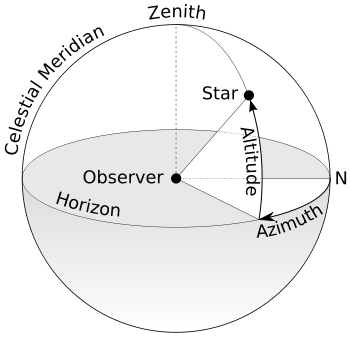
\includegraphics[scale=0.3]{azimuth.png}

\end{definition}

\begin{definition}[Bijection]
    \begin{align}
        S,R \text{\ are sets} \\
        \forall{i \in S}, \exists!{f(i) \in R} \wedge \\
        \forall{i \in R}, \exists!{f(i) \in S} \\
    \end{align}
\end{definition}

\begin{definition}[Boundary value problem]
    A differential equation with additional restrains. A solution to a boundary
    value problem is a solution to the differential equation which also
    satisfies the boundary conditions.
    
\end{definition}


\begin{definition}[Cauchy sequence]
    a sequence whose elements become arbitrarily close to each other as the
    sequence progresses.
    Think of \textit{two} curves that approximate each other.

\end{definition}

\begin{definition}[Cardinal number, ]
    The size of a set.
\end{definition}

\begin{definition}[Convergence]\label{convergence}
    A series is convergent is the sum of it's elements approaches a given 
    number.
\end{definition}

\begin{definition}[Convolution]
    Dictionary: a coil or twist, especially one of many.\newline
    Informal: an expression of how a shape from one function is modified by 
        the other.

    Can also be used to smoothen a discontinous a function (making it continous 
    on the given range). We need to normalize our g(x - $\tau$) so that we do
    not continously increase the f(x)
\end{definition}

\begin{definition}[Continuous]
In mathematics, a continuous function is a function for which
"small" changes in the input result in "small" changes in the output.

As an example, consider the function h(t), which describes the height of a
growing flower at time t. This function is continuous. By contrast, if M(t)
denotes the amount of money in a bank account at time t, then the function
jumps whenever money is deposited or withdrawn, so the function M(t) is
discontinuous.

\end{definition}

\begin{definition}[Continuous variables]
    There are three types of continuous variables:
    \begin{center}
    \begin{description}
        \item[Nominal] Categorized within groups: box 1, 2, 3 or 4.
        \item[Dichotomous] Boolean, yes or no.
        \item[Ordinal] A nominal variable, just that different groups give
            different values. E.g.\ to like something on a scale of 1 to 10
            gives you a ordinal range
    \end{description}
\end{center}
\end{definition}

\begin{definition}[Conjugate]
     is a binomial formed by negating the second term of a binomial. The
     conjugate of $x + y$ is $x − y$.

\end{definition}

\begin{definition}[Concave]
    Let $f$ be a function defined on the interval $[x_{1}, x_{2}]$.
    This function is concave according to the definition if, for every pair of
    numbers a and b with $x_{1} \leq a \leq x_{2}$ and $x_{1} \leq b \leq
    x_{2}$, the line segment from $(a,  f (a))$ to $(b,  f (b))$
    lies on or below the function.

    \begin{itemize}
        \item The sine function is concave on the interval $[0, \pi]$
        \item Concave if every line segment joining two point is never above
              the graph 
        \item Concave functions has $f\prime\prime(x) \leq 0$ in a given
              interval 
    \end{itemize}
\end{definition}

\begin{definition}[Congruence]
    Similar shape and growth, just different scalar / rotation.
\end{definition}


\begin{definition}[Damping]
    is an influence within or upon an oscillatory system that has the effect of
    reducing, restricting or preventing its oscillations. 
    Underdamped systems will start bouncy and then stop.

\end{definition}

\begin{definition}[Differential operator]
    An operator to do differentiation. This is mainly to abstract
    differenentiation.

\end{definition}

\begin{definition}[Discrete Fourier Transform]\label{dft}
    converts a finite list of equally spaced samples of a function into the
    list of coefficients of a finite combination of complex sinusoids, ordered
    by their frequencies, that has those same sample values.

\end{definition}

\begin{definition}[Discrete Laplace transform]
    An integral transfrom, which in 2d uses the kernel
    % \begin{bmatrix}   
    %     0 & 1 & 0 \\  
    %     1 & -4 & 1 \\ 
    %     0 & 1 & 0     
    % \end{bmatrix}     
\end{definition}

\begin{definition}[Discrete Sine Transform]
    Similar to~\nameref{dft}, but uses only a real matrix.

\end{definition}

\begin{definition}[Discretization]
    concerns the process of transferring
    continuous models and equations into discrete counterparts. 
    AKA\ smoothening curves to avoid jumps.

\end{definition}

\begin{definition}[Displacement]
    The shortest distance from source $s$ to $t$ (like air-distance).

\end{definition}

\begin{definition}[Divergence]\label{divergence}
    measures the magnitude of a~\nameref{vectorfield}'s source or sink at a
    given point, in terms of a signed scalar.

    E.g.\ air can be thought of to have a point $s \text{ and } t$, where they
    push out hot and cool air, respectively. From these points, you can create
    a~\nameref{vectorfield} that shows how air spreads from $s \text{ and }
    t$. The divergence measures the collected value from each of 
    these~\nameref{vectorfield}s.

    The operator for divergence is \verb|{div}|, represented by nabla.

    Given vector field $F = Ui, Vj, Wk$:
    \begin{align}
            div \textbf{F} = \nabla \cdot F = 
            \frac{\partial{U}}{\partial{x}}+
            \frac{\partial{V}}{\partial{y}} +
            \frac{\partial{W}}{\partial{z}}
    \end{align}

\end{definition}

\begin{definition}[Elementary function]
    In mathematics, an elementary function is a function of one variable built
    from a finite number of exponentials, logarithms, constants, and $nth$ roots
    through composition and combinations using the four elementary operations
    $(+ – × ÷)$.

\end{definition}

\begin{definition}[Expansion function]
    A function, with a series, to express a function. The series will in
    most cases be an approximation to the original function.
    Signal functions are often modeled using expansion functions.
\end{definition}

\begin{definition}[Eulers formula]
    $e^{ix} = \cos{x} + i\sin{x}$
\end{definition}

\begin{definition}[Explicit methods]\label{explicitmethod}
    In numerical analysis, an explicit method calculates the state of the system
    using only earlier history. See also~\nameref{implicitmethod}.
\end{definition}


\begin{definition}[Extreme point]
    A point furthest away from something.
\end{definition}

\begin{definition}[Field]
    A physcial quantity that has a value for each point in space and time.
\end{definition}

\begin{definition}[Finite difference]
    The difference in a function for $f(x + a) - f(x + b)$.

    There are three types:
    \begin{description}
        \item[Forward] is of the form $\bigtriangleup{f}(x) = f(x + h) - f(x)$
        \item[Backward] is of the form $\nabla{f}(x) = f(x) - f(x - h)$
        \item[Centered] is of the form $\delta{f}(x) = f(x + \frac{1}{2}h) - f(x - \frac{1}{2}h)$
    \end{description}
\end{definition}

\begin{definition}[Finite element method]
    (FEM) is a numerical technique for finding approximate solutions to
    boundary value problems for differential equations. It uses variational
    methods (the calculus of variations) to minimize an error function and
    produce a stable solution.  Analogous to the idea that connecting many tiny
    straight lines can approximate a larger circle, FEM encompasses all the
    methods for connecting many simple element equations over many small
    subdomains, named finite elements, to approximate a more complex equation
    over a larger domain.

\end{definition}

\begin{definition}[Filter bank]
    To take a signal and expose it to a series of filters that separate the
    input signal into different channel. One example is sound equalizers:
    you can adjust different parts of the signal.
\end{definition}

\begin{definition}[Fourier transform]
    Map one function onto another

\end{definition}

\begin{definition}[Fourier Analysis]
    the study of the way general functions may be represented or approximated
    by sums of simpler trigonometric functions

\end{definition}

\begin{definition}[Flow]
    Motion of particles in a given set.
\end{definition}

\begin{definition}[Generalized function]
   A distribution without steps, i.e.\ it is continious. 
\end{definition}

\begin{definition}[Harmonic numbers]
    $H_{n} = 1 + \frac{1}{2} + \frac{1}{3} + \dots + {1}{n} =
    {\sum\limits_{k = 1}^{k}} \frac{1}{k} \simeq \ln n$
\end{definition}

\begin{definition}[Heavyside Step Function]
    $$
    H(x) = \left\{
            \begin{array}{l l}
                0 & \text{for} x < 0 \\
                \frac{1}{2} & x = 0 \\
                1 & \text{for} x > 0 \\
            \end{array}
        \right.
    $$
    (it looks just like you think\dots)
\end{definition}

\begin{definition}[Homogenous]
    If a function $f$ is multiplied by a sclar $k$, then the result
    is a number multiplied by the scalar raised to some power $a$.
\end{definition}

\begin{definition}[Hyperbolic]
    Two curves that kind of face each other like bananas.
\end{definition}

\begin{definition}[Identity function]
    $\forall{x}, f(x) = x$
\end{definition}

\begin{definition}[Implicit method]\label{implicitmethod}
    In numerical analysis, an implicit method calculates the state of the system
    using both the current state and future ones. E.g.\ Gauss-seidel method
    See also~\nameref{explicitmethod}.
\end{definition}

\begin{definition}[Idempotence]
    An operation that can be applied multiple times without changing the
    the result. E.g.\ $f(f(x) = f(x)$
\end{definition}

\begin{definition}[Idenpendent variable]
    A variable that may be given without considering the value of other
    variables. E.g.\ for $y = 4x + 2$, x is indepdent (can be chosen freely)
    whereas $y$ is not: it depends on the value of $x$.
\end{definition}

\begin{definition}[Integral]
    The ``reverse'' to a derivate. 

    \begin{align}
        \int_{a}^{b}x^{n} dx = \frac{x^{n+1}}{n+1} + C \\
    \end{align}

    A function is said to be \textit{locally integrable} if it 's integral is 
    finite in a given domain.

    \textbf{Integration by parts:} $\int{u \times v dx} = u\int{v dx} - \int{u\prime{(v dx}}dx $

    Some identities:
    \begin{longtable}{|l|l|}
        $\int_{a}^{b}\cos{x} $ & $\sin{x} + C $ \\
    $\int_{a}^{b}\sin{x}$ & $-1 \times \cos{x} + C $\\
    $e^{x}$ & $e^{x} + C $
    \end{longtable}

\end{definition}

\begin{definition}[Integral transform]\label{inttrans}
    Input a function, and output another (using integrals).
    To do the transformation, one typically usues a \textit{kernel function} (e.g.\ 
    using a stencil in a grid).

    Usually, this is done to find a domain or function that is easier to compute
    on. 

    After completing the computations, one performs an inverse integral transform
    to translate back to the original domain.
\end{definition}

\begin{definition}[Interpolating polynomial]
    Given a set of points, define a function $f$ that intersects these points.
\end{definition}

\begin{definition}[Kronecker delta]
    A function for two variables, that returns 1 if the variables are equal,
    and zero otherwise.
    $$
    \delta_{i,j} = \begin{array}{ll}
        0 & if i \neq j \\
        1 & if i = j
        \end{array}
    $$
\end{definition}

\begin{definition}[Law of cosines]
    \begin{align*}
        v \cdot u = |v||u|\cos{\theta} \\
    \end{align*}
    Note that if $v, u$ are unit vectors, their lengths are both 1.
    We can then rewrite the expression as
    \begin{align*}
        v \cdot u &= \cos{\theta} \\
        \arccos{(v \cdot u)} &= \theta
    \end{align*}
\end{definition}

\begin{definition}[Laplace operator]
    Transform a function of $f$ of $t$ to a function $f$ of $s$

    A differential operator given by the~\nameref{divergence} of a gradient 
    function in euclidian space.
\end{definition}

\begin{definition}[Laplacian Matrix]
    sometimes called admittance matrix, Kirchhoff matrix or discrete Laplacian,
    is a matrix representation of a graph.

\end{definition}

\begin{definition}[Lattice]
    In mathematics, especially in geometry and group theory, a lattice in
    $\mathbf{R}^n$ is a discrete subgroup of $\mathbf{R}^n$ which spans the real
    vector space $\mathbf{R}^n$. Every lattice in $\mathbf{R}^n$ can be generated
    from a basis for the vector space by forming all linear combinations with
    integer coefficients. 

\end{definition}

\begin{definition}[Line integral]
    An integral where the function to be integrated is along a curve.
    The function is usually a~\nameref{vectorfield} or~\nameref{scalarfield}.

\end{definition}

\begin{definition}[Locus]
    a set of points whose location satisfies or is determined by one or more
    specified conditions

\end{definition}

\begin{definition}[Moment]
    TBD.
\end{definition}

\begin{definition}[Numerical analysis]
    The study of algorithms that use numerical approximation (as opposed to
    general symbolic manipulations) for the problems of mathematical analysis.

    Given a space $V$, find a finite subspace of $V$, such that you can
    calculate on it..

    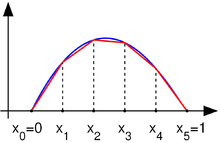
\includegraphics[scale=1.0]{fem.png}
    A function in  with zero values at the endpoints (blue), and a piecewise
    linear approximation (red)

\end{definition}

\begin{definition}[Odd function]\label{oddfunc}
    A function with the same values when you rotate 180 degrees around...
    \begin{align}
        - f(x) &= f(-x) \\
        f(x) + f(-x) &= 0
    \end{align}
    See also~\nameref{evenfunc}
\end{definition}

\begin{definition}[Even function]\label{evenfunc}
    Kind of like a mirror (90 degrees) around an axis;
    \begin{align}
        f(x) &= f(-x) \\
    \end{align}
    See also~\nameref{oddfunc}
\end{definition}

\begin{definition}[Pathological]
    Something that is counter-intuitive. The opposite is \textbf{well-behaved}.

\end{definition}

\begin{definition}[Parabola]
    A U-shaped, 2d, symmetrical curve.
\end{definition}

\begin{definition}[Parameterization]
    Represent a curve as a function.
    \begin{align}
        x = \cos{t} \\
        y = \sin{t}
    \end{align}
    is the parametric representation of a unit circle.

\begin{definition}[Partial derivative]
    Given a function $f$ with multiple parameters, a partial derivative is a
    derivative with respect to one of those variables.

    Partial derivatives are often denoted by $\partial$.

    To use partial derivation, you often assume that the other variables are 
    constants. Otherwise, there is an infinite number of tangent lines at
    any point, so you will have to have some range on the tangents.

\end{definition}

\end{definition}

\begin{definition}[Partial differential equation]
    A set of variables, and equations that show how they are all linked 
    together.
\end{definition}

\begin{definition}[Power series]\label{powerseries}
    \begin{align}
        f(x) = \sum\limits_{n=0}^{\infty}{a_{n}{(x-c)}^{n}}
    \end{align}
\end{definition}

\begin{definition}[Rectangle function]
    $$
    \Pi(x) = \left\{
            \begin{array}{l l}
                0 & \text{for} x > \frac{1}{2} \\
                \frac{1}{2} & \text{for} x = \frac{1}{2} \\
                1 & \text{for} x < \frac{1}{2} \\
            \end{array}
        \right.
    $$
\end{definition}

\begin{definition}[Reference value]
    The optimal/starting value. Note that when calculating differences,
    a reference value implies that order matters, i.e.\ $x - y \neq y - x$.

\end{definition}

\begin{definition}[Residual]
    In numerical analysis, this is the error from a result.
    E.g.\ in integration we have something-something + $C$, where C is the 
    the residual.

    It can (perhaps betterly) be stated that residuals is the error that occurs
    when approximating a function.

\end{definition}

\begin{definition}[Riemanns sum]\label{riemannsum}
    Sum from an integral. Divide the area under/over a curve into rectangles
    or trapezoids, and sum together their area. The smaller the shapes, the
    better.

    It is important to note that~\nameref{riemannsum} is an approximation - 
    one can not perfectly reconstruct the area under a curve.
\end{definition}

\begin{definition}[Risk function]
    Gives the expected value from a lossy function (compare two results, diff).
\end{definition}

\begin{definition}[Sine wave]
or sinusoid is a mathematical curve that describes a smooth repetitive
oscillation.

Its most basic form as a function of time $(t)$ is:

$y(t) = A\sin(2 \pi f t + \varphi) = A\sin(\omega t + \varphi)$
where:
\begin{description}
    \item[A], the amplitude, is the peak deviation of the function from zero.
    \item[f], the ordinary frequency, is the number of oscillations (cycles)
        that occur each second of time.
    \item[ω] = 2πf, the angular frequency, is the rate of change of the
    function argument in units of radians per second 
    \item[$\varphi$], the phase, specifies (in radians) where in its cycle the
        oscillation is at t = 0. I.e.\ the ``horizontal shift'' from a regular
        sine wave(????).
    If you e.g.\ represent two functions, $f(x) = \sin{x}$ and $g(x) = \sin{x} + 3$
    , the difference, i.e.\ phase shift, is 3. Note that these two functions
    have the same amplitude and frequency.
\end{description}

\end{definition}

\begin{definition}[Standard form]
    To write a number as a power of 10.
\end{definition}

\begin{definition}[Taylor series]
    A representation of a function as an infinite sum of terms that are 
    calculated from the derivatives at a point in the function.
    The formula is:
    \begin{align}
        \sum\limits_{n=0}^{\infty}{\frac{f^{(n)}(a)}{n!}{(x-a)}^{n}}
    \end{align}
\end{definition}

\begin{definition}[Shift invariant system]
    A discrete form of~\nameref{TIS} - the timesteps are discretized to follow
    a lattice spacing.
\end{definition}

\begin{definition}[Time invariant system]\label{TIS}
    A function with an output that does not depend on the output:
    \begin{align}
        x(t) &= y(t) \\
        x(t + \delta) &= y(t + \delta)
    \end{align}

    One example is the derivative function of polynomials (and others?) -
    no matter what timestep you choose - the value if the same.

    The ``antonym'' would be a time variant system.
\end{definition}

\begin{definition}[Translation invariant system]
    A system such that after a translation from A to T, any operator
    applied to A yields the same results in T.
\end{definition}

\begin{definition}[Unity]
    The number one. ``Unit functions'', ``unit circles'' all have the number 1.
\end{definition}

\begin{definition}[Univariate]
    An equation with only one variable.
\end{definition}

\begin{definition}[Vector Field]\label{vectorfield}
    An assigment of direction for a given set of points in an euclidian space.
    E.g.\ select every (10n, 10n) pixels in an image and get their derivative.
\end{definition}

\begin{definition}[Window function]
    A function that is zero outside of a given domain.
\end{definition}

\section{Graphs}

\begin{definition}[Arborescence]
    an arborescence is a directed graph in which, for a vertex u called the
    root and any other vertex v, there is exactly one directed path from u to v.
 \end{definition}

\begin{definition}[Clique]
    A subset of vertices $C \subset V$, such that in this subgraph all nodes
    are connected, i.e.\ there is an edge from every pair of nodes.
\end{definition}

\begin{definition}[Connected graph (component)]\label{connectedcomp}
    A graph in which, from any $v \in V$, you can reach any other $u \neq v$
\end{definition}

\begin{definition}[Directed graph]
    Properties:
    \begin{itemize}
        \item $\sum\limits_{v \in V}{d(v)} = 2|E|$
        \item $\sum\limits_{v \in V}{indegree(v)} = 
            \sum\limits_{v \in V}{outdegree(v)}$
    \end{itemize}
\end{definition}

\begin{definition}[Eularian]\label{eularian}
    Visit each \textit{edge} once.
\end{definition}

\begin{definition}[Hamiltonian]
    Visit each \textit{vertex} once.
\end{definition}

\begin{definition}[Metric spaces]\label{metric}
    See also~\nameref{semimetric}
    Properties:
    \begin{itemize}
        \item $d_{u,v} = 0 \iff u = v$
        \item $d_{u,v} = d_{v,u}$
        \item $\forall k, d_{u,v} \leq d_{u,k} + d_{k,v}$
    \end{itemize}
\end{definition}

\begin{definition}[Minimum mean cost]
    minimize ratio of cost of arcs (directed edges) to number of arcs
\end{definition}

\begin{definition}[MST]
    A mininum~\nameref{spantree}, such the weight of this tree is less than
    or equal to all other possible~\nameref{spantree}.
\end{definition}

\begin{definition}[Planar graph]
    No edges need to cross each other.
\end{definition}

\begin{definition}[Semi-metric]\label{semimetric}
    Like a~\nameref{metric}, without the property that
    $d_{u,v} = 0 \iff u = v$
\end{definition}


\begin{definition}[Spanning tree]\label{spantree}
    Connected, undriected graph that has all vertices and some subset
    of edges to form a tree.
\end{definition}

\begin{definition}[Strongly connected component]
    Similar to~\nameref{connectedcomp}, but in a directed graph.
\end{definition}

\begin{definition}[Topological sort]\label{topsort}
    Runs in O(V + E), same as DFS, although it can be supered to $O(\log_{2} n)$
\end{definition}

\begin{definition}[Tree]\label{tree}
    Properties of a tree:
    \begin{itemize}
        \item in a tree, there will always be an even amount of nodes that has
            an uneven degree.
        \item Degree of nodes in a tree is at most twice the number of nodes
    \end{itemize}
\end{definition}



\begin{definition}[Vertex-cover]
    A selection of vertices such that each edge is incident to at least one
    of them.
\end{definition}


\section{Image Processing}

\begin{definition}[Aliasing]
    Images are constructed and then reconstructed one or more times - 
    each of these reconstructions are referred to as aliases.
\end{definition}

\begin{definition}[Anisotropy]\label{anisotropy}
    Directionally dependent. Opposite of~\nameref{isotropy}.
    Example is to apply a filter to a set of images - consider
    what would happen if one image was tilted.
\end{definition}

\begin{definition}[Anisotropic diffusion]
    also called Perona-Malik diffusion, is a technique aiming at reducing image
    noise without removing significant parts of the image content, typically
    edges, lines or other details that are important for the interpretation of
    the image.

\end{definition}

\begin{definition}[Aperture]
    A hole which light goes through.
\end{definition}

\begin{definition}[Convolution]\label{convolution}
    In image-processing, this can in general be thought of as applying a mask
    that takes the local neighbourhood for a pixel x and calculates its
    gradient.

    Noteworthingly, convolution as an operation to an image is in general
    $O(n^{2})$.
\end{definition}

\begin{definition}[Dilation (of functions)]
    To skew a function, e.g.\ for $f(x) = x$, you skew to $\hat{f}(x) = x + 2$.
\end{definition}

\begin{definition}[Dirichet boundary condtions]
    In image processing, you can say that this boundary condition is to assume
    for a set of differential equations, the unknowns at the borders are 
    equal in the equations and image.

\end{definition}

\begin{definition}[extrapolation]
    The process of estimating, beyond the original observation range, the value
    of a variable on the basis of its relationship with another variable.

    Creating a tangent line at the end of the known data and extending it
    beyond that limit.

\end{definition}

\begin{definition}[Filter]
    Applying a mask or operation to an image to extract or distort values.

    \begin{description}
        \item[High-pass] takes only the high frequency into play, lower values
            are not affected that strongly (if at all)
        \item[Low-pass] \dots
    \end{description}
\end{definition}

\begin{definition}[Gaussian blur]
    Use a gaussian function on an image to reduce image noise and detail
\end{definition}

\begin{definition}[Gaussian filter]
    Gaussian filters have the properties of having no overshoot to a step
    function input while minimizing the rise and fall time.

\end{definition}

\begin{definition}[Gaussian pyramid]
    A stack of images, where for each iteration, you take neighboring pixels
    and make them into one. That is, you reduce the intensity in the picture.
    This compresses the image. 

    It is a pyramid because for each iteration you take neighboring pixels
    from the previous pyramid to generate the current.
\end{definition}


\begin{definition}[Gradient flow]
    $$
        V = \nabla{f} = \left(\
        \frac{\partial{f}}{\partial{x_{1}}},
        \frac{\partial{f}}{\partial{x_{2}}},
        \dots,
        \frac{\partial{f}}{\partial{x_{n}}}
    \right)
    $$

    Note that for an oridnary image, the gradient at a given position is 
    given by:
    $$
    \nabla{f} = 
    \frac{\partial{f}}{\partial{x}}\hat{x} +
    \frac{\partial{f}}{\partial{y}}\hat{y}
    $$
    Where the first (x) term is the gradient in direction x, and y is the
    gradient in direction y.

    One can also calculate the direction of the gradient using
    $\theta = a\tan^{2}{\frac{\partial{f}}{\partial{y}}, \frac{\partial{f}}{\partial{x}}}$
\end{definition}

\begin{definition}[Grating]
    A collection of identical pararell objects, placed next to each other with
    equal spacing.
    \end{definition}
\begin{definition}[Grayscale]
    an image in which the value of each pixel is a single sample, that is, it
    carries only intensity information

    Grayscale images are distinct from one-bit bi-tonal black-and-white images,
    which in the context of computer imaging are images with only the two
    colors, black, and white (also called bilevel or binary images). Grayscale
    images have many shades of gray in between.

    Grayscale images are often the result of measuring the intensity of light
    at each pixel in a single band of the electromagnetic spectrum 

\end{definition}

\begin{definition}[Image gradient]
    Gradual blend of color
\end{definition}

\begin{definition}[Image noise]
    Unwanted signal, electrical signals not wanted in an image
\end{definition}

\begin{definition}[Image masking]
    Apply an image over another. This can be used for e.g.\ putting a square image
    with only contents in the middle over another.
\end{definition}

\begin{definition}[Interpolation]
    A way to estimate (pixel) values when resizing to a larger image.

    An example from calculus is: given temps at noon and midnight, estimate
    the temp at 5 PM as the mean of noon and midnight.

    Interpolation can also (in signal processing) be referred to as 
    \textbf{upsampling}.

\end{definition}

\begin{definition}[Isotropy]\label{isotropy}
    Directionally independent. Opposite of~\nameref{anisotropy}.
\end{definition}

\begin{definition}[Laplacian]
    Highlight regions of rapid intensity change and is therefore often used for
    edge detection.

    Often applied to an image that has first been smoothed with something
    approxiating in order to reduce its sensitivity to noise.

\end{definition}

\begin{definition}[Spatial frequency]
    The number of changes in color values that occur per space.

    Images with high spatial frequency are detailed, images with low spatial 
    frequency will appear blurred.

    I.e.\ sharp transitions from low/high to high/low intensities are said
    to have a large spatial frequency,

\end{definition}


\begin{definition}[SRGB]
    sRGB is a standard RGB color space created cooperatively by HP and
    Microsoft in 1996 for use on monitors, printers and the Internet.

\end{definition}


\begin{definition}[Poisson image editing]
    Blend two images together and make them seem alike.
\end{definition}

\begin{definition}[Raster order]
    Begin at top left, proceed to right, then at leftmost pixel in next line.
\end{definition}

\begin{definition}[Raster image]
    An image with pixels.
\end{definition}

\begin{definition}[Ringing]
    The size of the oscillations after a peak frequency. E.g.\ if you have a 
    sudden overshoot (bright color) the amplitude of the next wave is
    the ringing. (???)
\end{definition}

\begin{definition}[Scalar field]\label{scalarfield}
    Associate a value to every point in a space. E.g.\ for an image, you
    could assign each pixel a color value.
\end{definition}

\begin{definition}[Seperable filter]
    A filter that can be written as the product of two or more small filters.
    This is usually done to reduce the computational costs.
    E.g.~\nameref{convolution} is usually faster in 1d than iterating $nD$, for
    $n \ge 2$.
\end{definition}

\begin{definition}[Stencil]
    A figure that connects dots on a grid. Usually a cross-like figure 
    (one center dots, and one edge out in 4 directions from the center to
    other dots).
\end{definition}

\section{Linear Algebra}

\begin{definition}[Basis]
    Given a set of vectors in $\mathbf{R}^{n}, V$, which is linearly
    independent, the set $V$ is a \textit{basis} if you can span 
    $\mathbf{R}^{n}$ using $V$.
\end{definition}

\begin{definition}[Condition number]
    A measure of how the output value for a function changes respective to 
    input variables.
\end{definition}

\begin{definition}[Column space]
    All linear combinations of the columns of a matrix $A$.
\end{definition}

\begin{definition}[Consistent]
    $\iff$ the rightmost column of an augmented matrix is not a pivot column.
    I.e.\ in a 3x4 matrix, if the last row is zero and 2nd column has pivot
    column, then the system is still consistent.
\end{definition}

\begin{definition}[Diagonal Dominance]
    $\forall{i}, \exists{i} A_{i, i}, \forall i, \iff A_{i,i} 
    \geq \sum\limits_{j = 0, j\neq i}^{m}$,
    then matrix $A$ is DD.
\end{definition}

\begin{definition}[Dotting matrices]
    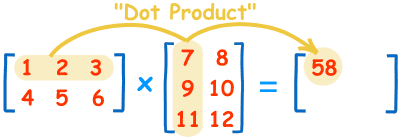
\includegraphics[scale=0.3]{mm.png}
\end{definition}

\begin{definition}[Eigenvector]\label{eigen}
    Given a square matrix A, when A is multiplied with an eigenvector $v$,
    the resulting matrix A${^\prime}$ is a multiple of $v$.
    The multipe is denoted by $\lambda$ and is called an eigenvalue.
    So, $Av = \lambda v$

\end{definition}

\begin{definition}[Gaussian Elimination]
    AKA ``Row reduction''. Add row $x$ to row $y, y \neq x$, to reduce $y$ to 
    zeroes.

\end{definition}

\begin{definition}[Inverse]
    For a matrix $A \in \mathbf{R}^{2x2}$:
    $A^{-1} = \frac{1}{|A|}
        \begin{bmatrix}
            d & -b \\
            -c & a
        \end{bmatrix}
    = \frac{1}{ad - bc}
        \begin{bmatrix}
            d & -b \\
            -c & a
        \end{bmatrix}
    $\\
    For a matrix $A \in \mathbf{R}^{3x3}$: bcacab

    Properties:
    \begin{itemize}
        \item $(A^{-1})^{-1} = A$
    \end{itemize}
\end{definition}

\begin{definition}[Kernel]
    For a vector space given by a~\nameref{lintrans}, a kernel is the set
    of vectors $v \in V$, s.t. $T(u) = 0$.
\end{definition}

\begin{definition}[Length of Vector]\label{vectorlength}
    For a vector 
    \begin{align*}
        v = [a_{1}, a_{2}, \dots , a_{n}] \\
        |v| = \sqrt{a^{2}_{1} + a^{2}_{2} + \dots + a^{2}_{n}}{}
    \end{align*}
\end{definition}

\begin{definition}[Linear dependence]
    For $V = {v_{1}, \dots, v_{n}}$, and $\forall v, v is vector$,
    if none of the vectors in V can be written as a linear combination
    from the other vectors in V, the set is linearly independent.
\end{definition}

\begin{definition}[Linear transformation]\label{lintrans}
    Take a vector space into another, s.t.\
    \begin{align}
        T(u + v) = T(u) + T(v) &\forall u,v \in v \\
        T(cu) = cT(u) &\forall u \in V
    \end{align}
\end{definition}

\begin{definition}[Norm]
    The ``length'' of a vector, just remember to sum up over all dimensions.
    Each number is raised to $n$, and the total sum is then raised to
$\frac{1}{p}$.  \end{definition}

\begin{definition}[Normalization of vectors]
    $ \hat{X} \equiv \frac{X}{|X|} $, where $|x|$ is the~\nameref{vectorlength}
    $X$ is, in this case, evaluated as the additive sum of it's entries.
\end{definition}

\begin{definition}[Null space]
    Given a matrix $A$, if you solve for that each row = 0,
    all possible values for each $x$ makes out the Null space.

    Note that here it is apossible to get free variables for 
    some x, and bound to others.

\end{definition}



\begin{definition}[Orthogonal]\label{orthogonal}
    Two lines that intersect each other at 90 degrees.\\
    \begin{itemize}
        \item Orthogonal matrices preserve dot products:
        given two vectors $u$, and $v$, and an orthogonal matrix Q,
        the following is true:
        $u \times v = Qu \times Qv$
        \item The determinant of an orthogonal matrix is always 1 or -1
        \item The transpose of $Q$ is equal to it's inverse, hence:
            $Q \times Q^{T} = I$
    \end{itemize}
\end{definition}

\begin{definition}[Perpendicular]
    Similar to~\nameref{orthogonal}, but with lines.
\end{definition}

\begin{definition}[Plane]
    A flat, two-dimensional surface
\end{definition}

\begin{definition}[Positive semidefninite matrix]
    Properties:
    \begin{itemize}
        \item Nonnegative~\nameref{eigen}s
        \item $X = V^{T}V$ for some $V \in \mathbf{R}^{mxn}$
        \item $X = \sum\limits_{i=1}^{m}\lambda_{i}w_{i}w^{t}_{i}$ 
            for some $\lambda_{i} \geq 0$ and vectors $w_{i} \in \mathbf{R}^{n}$
            such that $w^{T}_{i}w = 1$ and $w^{T}_{i}w_{j} = 0$

    \end{itemize}
\end{definition}

\begin{definition}[Projection]
    define a vector $v$ and $u$.
    \begin{align*}
        L &= \left\{cv | c \in \mathbf{R} \right\}  \\
        proj(v) &= l \in L \text{\ such that\ } u - proj(v) 
        \text{\ is~\nameref{orthogonal} to l}  \\
        \textit{I.e., } proj(v) &= cv, c \in \mathbf{R}
    \end{align*}

    Properties:
    \begin{itemize}
        \item $proj(v) = proj(v)^{2}$
        \item Linear independence on $u, v$ also relates for $v - proj(v), u$
        \item adding $proj(v)$ to $v$ gives you $u$
    \end{itemize}

\end{definition}

\begin{definition}[Span of vectors]\label{vectorspan}
    All linear combinations of a set of vectors.
    \begin{align*}
        V &= \left\{v_{1}, \dots, v_n\right\} \\
        C &= \left\{c \in C | \mathbf{R}\right\} \\
        span &= c_{1}v_{1} + \dots + c_{n}v_{n}
    \end{align*}
\end{definition}

\begin{definition}[Spectral Radius]
    The largest eigenvalue of a matrix.
\end{definition}

\begin{definition}[Symmetric]
    \begin{itemize}
        \item Length of rows is equal
        \item The transpose is equal to the originl
    \end{itemize}
\end{definition}

\begin{definition}[Tensor]
    Geometric objects that describe linear relations between vectors or scalars.
\end{definition}

\begin{definition}[Trace]
    Sum of all diagonal entries in a matrix.
    $A_{11} + A_{22} + A_{nn}$
\end{definition}

\begin{definition}[Transpose]
    Take column $i$ and make it into a column. Repeat.
\end{definition}

\begin{definition}[Unit vector]
    A vector who's length is 1.
\end{definition}


\begin{definition}[vector length]
    number of "steps" in a vector
\end{definition}


\begin{definition}[Information space]
    is the set of concepts and relations among them held by an information
    system; it describes the range of possible values or meanings an entity can
    have under the given rules and circumstances.

\end{definition}

\section{Programming Security}

\begin{definition}[Accessory controls]
	If a company X notices that a part P of a product does not belong to them,
	they may reduce the effectiveness of the product.

	For example, if a printer notices a competitors ink in the printer, it 
	may go from high quality to low.

	This is considered a form of authentication.
\end{definition}

\begin{definition}[Access control]
	I assume the meaning is intuitive to understand.
	What's worth mentioning is that access control can operate on four levels,
	namely:
	\begin{itemize}
		\item Application
		\item Middleware
		\item Operating system
		\item Hardware
	\end{itemize}
\end{definition}

\begin{definition}[Access Control Lists]\label{ACL}
	Most UNIX-fans will know them already: 
		\textit{-rw-r--r-- 1 $<$owner of file$>$ $<$group owner of file$>$.}
	This is an example of a rowwise mandatory ACL- where an object
	has a given set of definitions for three different groups:
	the first three letters in the string denotes what the owner can do
	(in this case, there is no execution, but read and write),
	the third next letters (mid-block) denote what members of the
	owner group can do to the file, and the next three letters denote
	what everyone else can do.

	This type of ACL are slow for systems with many users. 
	The vantage is that is efficient. Other forms of ACL's include
	database access control (suffering from inability to model
	states, etc.
\end{definition}
\begin{minipage}{\linewidth}
\makebox[\linewidth]{% center the image
  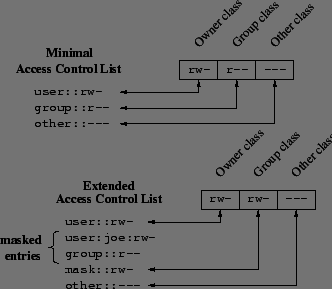
\includegraphics[keepaspectratio=true,scale=0.6]{./ACLnix.png}}
  \captionof{figure}{Typical UNIX ACL}% only if needed
  \label{visina8}

\end{minipage}

\begin{definition}[Assurance classes]
\end{definition}

\begin{definition}[Authentication]
	To prove that you are who you claim to be. E.g.\ to provide a password
	for an account, etc.
\end{definition}

\begin{definition}[Authorization]

	To ensure that a user has sufficient permissions to do what he/she
	asks for. E.g.\ an authenticated user may log in, but may not
	change the passwords for other users, because this authenticated user
	is not authorized for this account.
\end{definition}

\begin{definition}[BAN-logic]
	IS THIS REALLY NECESSARY?

	\dots formal reasoning in cryptology, somewhat alike first-order-logic.
\end{definition}

\begin{definition}[Biba Model]\label{biba}
	Essentially BLP, just that it is read by "no read down, no write up".
	The BLP can be categorized as "no write down, no read up".

	\epigraph{A monk may write a prayer book that can be read by commoners, 
	but not one to be read by a high priest}
	{--- \textup{Wikipedia}}

\end{definition}

\begin{definition}[Bell LaPadula model]
	Any system that adheres to the two following properties, are said to
	adhere to the Bell LaPadula Model, which is a \nameref{secpol}:
	\begin{description}[labelindent=1cm]
		\item[Simple security property] 
			\textit{no process may read data at a higher level.}
			If a process is on runlevel X, it should not have access to data at level 
			X + 1.
		\item[*-property]
			\textit{no process may write data to a lower level.} Imagine 
			that a sysadmin gets a Trojan that reads much sensitive data. 
			The *-property prevents this data to be written down to a lower level
			where it is accessible to other accounts with lower clearance.
	\end{description}

	It is worthwile noting that the properties fail to mention policies
	for creation and destruction of files.
	Furthermore, the model is broken if sensitive data is temporarily declassified. 
	The data can then be manipulated without violating the constraints of BLP.\
	Hence, to make the BLP safe, we need to introduce the 
    \textbf{tranquility property}:
	\begin{description}[labelindent=1cm]
		\item[Strong:] 
			Security labels on objects never change during systems operation.
		\item[Weak:]
			Security labels never change in such a way that it defines the
			given security policy.
	\end{description}

	However, the problem with the tranquility property is that process will 
	have a difficult time reading files. If at first one reads something at 
	a high level, then no concurrent read/write operation can occur for a lower
	level. Applications will therefore need to be customized extensively to accomodate
	for the tranquility property.

	The BLP only deals with confidentiality, not integrity (see~\nameref{biba})
\end{definition}

\begin{definition}[Biba Model]
	Deals with integrity alone, ignores confidentiality.
\end{definition}

\begin{definition}[BMA model]
	British Medical Association. 
	Basically a 9-point long list wich comprehends the BLP,
	but also represents state, and so on. Used for medical records.

	It's worthwhile noting that for medical records, it's much harder to
	define privacy and such because doctors are often required to involve
	third parties with their records. This could be researchers, drug companies,
	family, so on.
\end{definition}

\begin{definition}[Capture error]
	People are used to clicking "OK" on alert boxes without reading, so you
	might fool them intro clicking on one of your buttons by simply 
	making a popup box.
\end{definition}


\begin{definition}[Chinese Wall]
	Lets say that you work in finance, reviewing different oil companies.
	If you've worked on account A for some time, you might have information
	that is relevant for account B. To prohibit this, you're given
	a timed restriction, such that you cannot work on other accounts 
	if you have sensitive information.

	The general idea is to say that "you can access this, but nothing else,
	there's a chinese wall between you and other accounts."

	The chinese wall has been expressed to be similar to the BLP.\
	Let $c$ denote objects of interest, for example bank data. $s$ 
	denotes a subject, for example a person, who tries to access objects.
	$y(x)$ is a function $y$ for an object $x$ that denotes a company $y$'s 
	interest for the object $x$. Similarily, for a company $f$, there's a 
	function $f(x)$. The domain $S = S(s)$ is a set which covers all
	objects that $s$ can access.

	\begin{description}[labelindent=1cm]
		\item[Simple security property]
			$\forall s$, $s$ will have access to $c$ iff $\forall o \in S(s)$
			, $y(c) \cap x(o) = \emptyset$ or $y(c) \in y(o)$
		\item[The *-property]
			$s$ can write to an object $c$ iff $\forall o\{m \| m \in S(s) \} ),
			o \notin x(c) $ and $y(c) \neq y(o)^{[what?]}$
	\end{description}
\end{definition}

\begin{definition}[Common Criteria]\label{cc}
	Defines many~\nameref{secfunreq}. ISO-standard.
\end{definition}

\begin{definition}[Confidentiality]
	\textit{Who/what could have read this message?}
\end{definition}

\begin{definition}[Covert channel]
	If a system adheres to the BLP, a low security object might still
	commuicate with one at a higher level. If the two share a resource,
	e.g.\ a disc, one could make the higher level process do something
	with the disc head to communicate. This could for example be invoking 
	an error at time $t_{i}$ to indicate that bit $i$ in an important file is
	either 1 or 0. This way of communication is called a covert channel.
\end{definition}


\begin{definition}[Cryptographic nonce]\label{nonce}
	a nonce is an arbitrary number used only once in a cryptographic communication.
	The nonce is there to ensure freshness of a message, e.g.\ it could be a
	timestamp. That way, one can be assured that encrypted messages are
	recent and not old.
\end{definition}

\begin{definition}[CSRF]
	performs an action on the server. The user is typically not aware 
	of what he/she is doing. I.e., if there is a URL that can be used
	to purchase 50 cars, Eve can send that to Alice and make her, unwillingly,
	buy 50 cars.

	CSRF attack can be mitigated by properly implementing session authentication
	tokens, such that one cannot modify/use an account without having a 
	valid token from the server. That way, the POST to purchase cannot be
	instantiated unless the client performs a series of steps.
	$\qedhere$
\end{definition}

\begin{definition}[Discretionary Access Control]\label{DAC}
	A simple form of access control. The ease of implementing DAC makes it popular.
	DAC is similar to~\nameref{mac}, except
	from that there are no \textit{policies} for objects. This means that
	whenever a subject wants to apply an action to an object $o$,
	the operating system will only evaluate $s$ and $o$, not the action that $s$ wants 
	to apply, in order to determine whether or not $s$'s action will be executed.
\end{definition}

\begin{definition}[Difference between DAC and MAC]\label{diffDACMAC}
	DAC is not a multilevel security protocol in that, for any subject 
	$s$, \textbf{any} operation on an object $o$ is either granted or not 
	\textbf{only by considering the relationship between $s$ and $o$, not
	the action applied}.
	
	Furtherly, the following quotes quite sum it up:
		\epigraph{Systems can be said to implement both MAC and DAC simultaneously,
		where DAC refers to one category of access controls that subjects can 
		transfer among each other, and MAC refers to a second category of access 
		controls that imposes constraints upon the first.}{--- \textup{Wikipedia}}

		\epigraph{In general, when systems enforce a security policy independetly 
		of user actions, they are described as having madatory access control,
		as opposed to the discretionary access control in systems like Unix where 
		users can take their own access decision about their files}
		{--- \textup{Page 246 in the book}}
\end{definition}

\begin{definition}[Evaluation Assurance Level]
The~\nameref{cc} uses 
\end{definition}

\begin{definition}[Format string vulnerability]
	Input data will be used to format output. However, the input data
	goes to the stack, and there are therefore vulnerabilities.
\end{definition}

\begin{definition}[High water mark principle]
	Start off at the bottom and elevate permissions as you need them.
	E.g.\` as one opens a mail client, one finds 
\end{definition}

\begin{definition}[Identify Friend or Foe]{IFF:}\label{iff}
	A system that can tell whether you are a friend of a foe.
	A classical crypto-problem; how can I know that I am not talking to Eve?
\end{definition}

\begin{definition}[Integer manipulation attack]
	Causing an under- or overflow or truncation such that you can 
	exploit software.
\end{definition}

\begin{definition}[Integrity]
	\textit{Who/what could have altered this package?}
\end{definition}

\begin{definition}[Kernel bloat]
	E.g.\ in Windows, you need to have many drivers run as root in the kernel.
	This will naturally open up for more security holes. 
\end{definition}

\begin{definition}[Key-distribution]\label{keydistribution}
	One entity on a network wants to talk to another in a network. 
	We will assume Alice wants to talk to Bob.
	Her concern is that they might establish a connection,
	but Eve might hijack it and pretend to be either party. Alice needs to know
	that she is speaking with Bob, and she needs to know that Bob is not 
	communicating with any Eve.

	To prevent this, a trusted third party is introduced. We will call this Sam.
	We will assume that the connection to Sam is safe, and that Sam knows 
	every user of the network.
	Alice contacts Sam. Her request is as follows: "I am Alice, and want to 
	communicate with Bob". Sam returns two tokens. The first token 
	can only be read by Alice, and the second only by Bob. Alice then contacts 
	Bob, giving him only the second certificate. Bob decrypts the certificate,
	which unravels an encryption/decryption key. Bob and Alice can now 
	encrypt and decrypt messages to each other using this key, and communicate
	without Sam.

\end{definition}

\begin{definition}[Landing pad]
	A piece of code, such that when exectued, the processor
	will exectue malicious code.
\end{definition}

\begin{definition}[Lattice model]
    Essentially equivalent to the BLP.\ You use labels such as "TOP SECRET",
    "SECRET" and say that there are no communications between levels as in the
    BLP.\

    You combine things, so for each item, e.g.\ for "missiles" you might have a
    clearance for something like "SECRET". But you also need codewords, such as
    "SECRET MISSILES" if you want to read the
	secret stuff about missiles.

    The point of the lattice model is that you have aggregated values, such
    that a lattice will yield a numeric $d$. To get access to $d$ you need $e >
    d$.
\end{definition}

\begin{definition}[Malware]
\end{definition}

\begin{definition}[Mandatory Access Control]\label{mac}
	\textit{Also known as multilevel security}.
	MAC is enforced as follows: for each object $o$, define a set of 
	actions that are applicable to this object, and categorize them by access level. 
	E.g.\ one could define deletions as \textit{administrator-level} and modifications as 
	\textit{user-level}. The categorization of actions to objects is known as
    defining the \textbf{policy}. The policy is often stored as
    an~\nameref{ACL}.  Typical values for $o$ include files, directories,
    ports, etc.  When subject $s$ requests an action $a$ on $o$, the operating
    system looks up the rules for $o$, finds $a$, and evaluates $s$ against the
    policy for $a$ on $o$.

	To clarify: in MAC, there is no such thing as "super-user-access", i.e.\
	being a user with high privileges won't necessarily grant you privileges on all
	objects, because some objects might have policies that only permit certain
	other users to manipulate them. For example, even though you might
	be a system administrator, you should not be able to read other user's
	passwords, nor modify them. You might rather grant sysadmins the privilege
	to reset the password, and let authenticated users modify their own passwords.

	MAC ensures a security policy indepent of user actions. That is, 
	even though a user owns a file, he/she might not be able to do 
	whatever he/she wants with it.
	
	A good example of the usefulness of MAC is that a computer that is hacked
	may not jepordize other systems. Despite of having obtained some level
	of control, the attacker may not get access to other critical features.

	MLS's are usually difficult to implement. One example is the 
	\textbf{cascading} problem; two systems A and B may both have access to an object $o$.
	Simeltaneously, system A have access to another object $a$, system B
	has access to object $b$, where $ a \neq b$. Now, modifying $o$ might
	affect how $a, b$ are treated. So if system B wants to alter
	$a$, it may modify $o$, then system A reads $o$, then modifies $a$.

	Do also note figure~\ref{xkcdauth} as it highlights a security
	caveat of MLS; low-level data can also be worthwhile protecting.
	See also the quote in \nameref{diffDACMAC}
\end{definition}
\begin{minipage}{\linewidth}
\makebox[\linewidth]{% center the image
  
\includegraphics[keepaspectratio=true,scale=0.6]{./xkcd_auth.png}}
  \captionof{figure}{xkcd.com/1200}% only if needed
  \label{visina8}
\end{minipage}\label{xkcdauth}


\begin{definition}[No-operation]{NO-OP:}
	From assembly, do nothing. 
\end{definition}

\begin{definition}[Phishing]
	Essentially the same as~\nameref{pretext}ing, just that you're trying to
	decieve customers instead of staff.
\end{definition}

\begin{definition}[Pretext]\label{pretext}
	To create a plausible scenario that can decieve personell with 
	sensitive information to disclose this to Eve.
\end{definition}

\begin{definition}[Principle of least privilege]
	Programs should only have as much privilege as they need.
	There's no need to "sudo webbrowser"

\end{definition}

\begin{definition}[Protection profile]
	A document that identifies the desired security properties of a product.
	This is structured as a list of security requirements defined 
	in a way that adheres to~\nameref{cc}
\end{definition}

\begin{definition}[Pump]
	A one way transfer (data diode) that takes data from
	a low access level to a higher access level. 
\end{definition}

\begin{definition}[Race condition]
	Process A reads resource X, process B reads resource X,
	process A writes, then process B writes. The value is bad, since B's
	original value was bad.
\end{definition}

\begin{definition}[Reflection attacks]
	First, see~\nameref{chalres}.
	Suppose that the challenge-response is similar for two
	entities. I.e.\ party A sends a challenge $N$ to someone.
	To solve the challenge, party E simply returns $N$ to $A$,
	has party A solve it, and voila, party E knows the solution to $N$.
\end{definition}

\begin{definition}[Replay attack] 
	Assume that to login, Alice encrypts her password with one million bits
	, three times, and sends her password to a login page. The login
	decrypts and accepts Alice's authentication token.

	Eve could simply sniff the POST from Alice and the replay it to the 
	server. Even though the password is highly encrypted,
	Eve's POST will be valid. The login page accepts Eve.

    To mitigate, one should/could implement session tokens;
    see~\nameref{sessiontoken}. As mentioned in that section, however, session
    tokens also introduce other risks.
\end{definition}

\begin{definition}[Repudiation attack]
	To give someone a bad reputation. This could be by rating items
	with low scores, writing mean reviews, etc.
\end{definition}

\begin{definition}[Role based access control]
	Permissions are not related to users, but rather their functions. 
	This means that if a sysadmin is sick, a second-in-rank user could
	assume the rank of the sysadmin to do whatever is necessary.
\end{definition}

\begin{definition}[Sandbox]
	A limited environment. It is common to host websites in sandboxes,
	so that even if the webserver is hacked, a hacker can't do much on the
	mainframe.
\end{definition}


\begin{definition}[Security Policy (model)]\label{secpol}
\end{definition}



\begin{definition}[Secrecy]
\end{definition}

\begin{definition}[Security assurance requirements]

\end{definition}

\begin{definition}[Security functional requirements]\label{secfunreq}
	
\end{definition}

	\epigraph{A document that expresses clearly and consicely what the 
	protection mechanisms are to acheieve. \dots It will often take the form of 
	statements about which users may access which data}{--- page 240}

	As with most computer policies, it's important the statements
	are succint, i.e.\ briefly and clearly expressed, without implications. 
	Also, it's important to make sure that you explicitly define:
	\begin{itemize}
		\item Who determines the policy?
		\item What qualifies for "need to know"?
		\item How will the policy be enforced?
	\end{itemize}

\begin{definition}[Security requrement]
	A statement which defines what level of security is utilized
	for different kind of attacks.
	It's important that the requirements do not discuss design,
	only what is required (hence, requirement).

	All requirements should be testable. Good ways to do this is 
	to quantify. Quantifying security is difficult, however.
\end{definition}

\begin{definition}[Security target]
	A document that describes what a product does, 
	or at the very what it does that has an impact/relevance in security contexts.
\end{definition}

\begin{definition}[Session token]\label{sessiontoken}
	\textit{Also known as session ID or session identifier}. 
	A session token is a unique identifier, usually in the form of a hash
	generated by a hash function that is generated and sent from a server to a 
	client to identify the current interaction session.	
	
	If Eve can obtain the session ID, she can also, in theory, perform 
	actions, pretending to be the victim. This is known as \textbf{session hijacking}.
	As the session ID needs to be submitted for every POST and GET, it can
	be easy to obtain it by sniffing or tricking the victim. Hence, there
	should also be other security measures in place to make the use of session
	tokens safe.
\end{definition}


\begin{definition}[Smashing the stack]
	Making an overflow such that excess bytes are considered as code 
	rather than arguments.
\end{definition}

\begin{definition}[Software Security Touchpoints]
\end{definition}


\begin{definition}[SQL-injection]
	If you can't define this, please go get some sleep.
\end{definition}

\begin{definition}[Target of Evaluation]{ToE.}
	The product under evaluation.
\end{definition}

\begin{definition}[Trojan]
	A piece of software that looks cool, but in reality it causes harm
	when executed.
\end{definition}

\begin{definition}[Two-channel authentication]
    I fail to see the big differnece from~\nameref{twofactor}
	but accoding to the book, this is "sending an access code the user
	via a separate channel"
\end{definition}

\begin{definition}[Two-factor authentication]\label{twofactor}
	To authenticate, you need "something you have, and something you remember".
	E.g.\ a password and a password calculator.

	Most companies are sceptical of this. While it does seem to improve
	security per today's date, it is still prone to real-time mitm attacks.
\end{definition}


\begin{definition}[validation of input]\label{validation}
	Given input $\iota$, filter any bad input $b$ and return $\iota_{clean}$
	There are multiple types of input validation:
	\begin{description}[labelindent=1cm]
		\item[Blacklist-validation] do not regard context and trim away any bad 
			characters from input. 
			I.e.\ one can define a set of bad characters in a set
			$S = \{ ' , " , \ \}$, etc. Given input $\iota$, return 
			$\iota_{clean}$, s.t. $\iota_{clean} \cap S = \{\emptyset\}$
			The problem with black-validation is that is often easily bypassed,
			since the attacker can often distort his input in a way that bypasses
			the filters. Note that the filter only checks for characters, not context.
		\item[Whitelist-validation]
			In many contexts, the character ' is considered malicious, however,
			it is also required in some names, etc. White-validation looks
			at what structure input should have, and validates accordingly.
			It is stronger than blacklist-validation in that, for example 
			for dates it is possible to know what structure the input should have
			, and thereby you can trim from character length and structure.

			It is also worhtwile to talk of this as contextual encoding.
	\end{description}
	
	Another form of validation is the translation of characters to another typeset.
	This is typically known as \textbf{escaping} input. Before using any
	input one can e.g.\ do html-escaping. I assume the reader knows what this is.
	Character escaping has a recommended order: first do HTML-escaping, then
	JS-escaping. Finally, it is worth mentioning about escaping that it 
	does not prevent XSS, it just makes it harder to render data as code$^{[why?]}$.
\end{definition}

\begin{definition}[Valet attack]
	Assume that you use a random number in your key to unlock something, 
	like a car. This means that whenever you want to unlock the car, there
	are different codes, all valid. 
	
	If Eve gets to unlock Alice's car every day, Eve can record all keys used
	to unlock Alice's car. Eventually, when Alice's car run out of memory,
	it will not remember that the first key has ever been used. Eve
	then tries to use this first key that she recorded. This unlocks the car.
\end{definition}

\begin{definition}[Virus]
\end{definition}

\begin{definition}{XSS}
	upload a script that to a server that will be executed by other users.
	XSS is a popular type of attack and hence there's a lot of 
	terminology\dots
	\begin{description}[labelindent=1cm]
		\item[Stored XSS] the malicious script sent by an attacker is stored
			permanently on the webserver.
		\item[Reflected XSS] the malicious script sent by an attacker 
			causes an immediate malformed response from the server, but
			the script will not be stored on the server.
		\item[DOM-based XSS] typically sends a URL to a user such 
			that his/her site, i.e.\ DOM, is modified. E.g.\
			if the values for a selection field is specified from the url,
			modifying the parameters to be scripts instead
			means that the DOM is modified via XSS.
	\end{description}
	\epigraph{Reflected and Stored XSS are server side
	execution issues while DOM based XSS is a client (browser) side 
	execution issue}{--- \textup{OWASP}, https://www.owasp.org/index.php/DOM\_based\_XSS\_Prevention\_Cheat\_Sheet}
	

	Mitigations: see~\nameref{validation}
\end{definition}

\section{Statistics}

\begin{definition}[Bernoulli distribution]\label{bernoulli}
    A distribution of parameters, where $\forall x, 0 \leq x \leq 1$,
    Typically dual, e.g.\ in coin toss there is heads and tails.
    If $\Pr_{heads} = k$, then $\Pr_{tails} = 1 - \Pr_{heads}$
\end{definition}

\begin{definition}[Bigvee]
    $\bigvee\limits_{a \in I} P_{a}$ says that at least one $P_{a}$ is true.
    It can also be used for the maximum value in a set.
\end{definition}

\begin{definition}[Chernoff bound]\label{chernoff}
    In a nutshell, it determines a bound on how many times we must perform
    a trial to know that our random variables represent a majority.
    E.g.\ if we trying to determine that a coin is biased (heads/tails),
    a chernoff bound will say how many times we must flip the coin to know
    that we have unraveled a bias. In this case, for example, simply flipping it
    twice will not suffice.
\end{definition}

\begin{definition}[Conditional expectations]
    $$
        E(X | Y=y) = \sum\limits_{x \in X} x \
        P(X=x | Y=y) = \sum_{x \in X} x 
        \frac{P(X=x,Y=y)}{P(Y = y)}
    $$
\end{definition}

\begin{definition}[Conditional probability]
    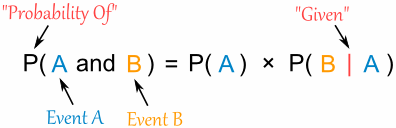
\includegraphics[scale=0.3]{prob_form.png}
\end{definition}

\begin{definition}[Expected value]\label{expectedvalue}
    $E[X] = \sum\limits_{s \in S}^{\dots} X(s) \cdot \Pr(\{s\}) $ \newline
    $E[X] = \sum\limits_{s \in S}^{\dots} X(s) \cdot \Pr(X = x) $
\end{definition}

\begin{definition}[hyperplane]
    A plane (surface) that has one less dimension than it's ambient space,
    i.e.\ the space around it. E.g.\ a hyperplane for 3-d dims is only defined
    2D.

    A hyperplane will therefore act as a separator. Imagine a holding a 
    square in the middle of a ball.
\end{definition}

\begin{definition}[Indicator variable]
    Indicator variable: 0 or 1 for whether an element is selected or not.
\end{definition}


\begin{definition}[Linearity of expectation]\label{lin_expect}
    $ E[X] + E[Y] = E[X + Y] \newline
    [\sum\limits_{x \in S}^{\dots} X(s) \cdot \Pr(X = x) +
    \sum\limits_{y \in S}^{\dots} X(s) \cdot \Pr(Y = y) ] \newline
    = [\sum\limits_{s \in S}^{\dots} a \cdot \Pr(Y = a) + a \cdot \Pr(X = a) ]
    $
\end{definition}

\begin{theorem}[Likelyhood that both X and Y occur in S]
    $ \newline E[X] \cdot E[Y] = E[X \cdot Y]$
\end{theorem}
\begin{proof}
    From~\nameref{expectedvalue}: \newline
    $
    E[X \cdot Y] = \newline \sum\limits_{z \in S}^{\dots} z \cdot 
        \Pr(X = z \text{ and } Y = z) = \newline
    \sum\limits_{x \in S}^{\dots}\sum\limits_{y \in S}^{\dots} x \cdot y
    \cdot \Pr(X = x \text{ and } Y=y) = \newline
    [\sum\limits_{x \in S}^{\dots} x \cdot \Pr(X = x)] \cdot  
    [\sum\limits_{y \in S}^{\dots} y \cdot \Pr(Y = y)]  = \newline
    E[X] \cdot E[Y]
    $
\end{proof}

\section{Operation Research}
\begin{definition}[Corner point feasible solution(CPF]
A solution that lies at the corner of a feasible region (solution space)
If a solution has only one feasible solution, it must be a CPF
\end{definition}

\begin{definition}[Feasile region]
    Aka solution space. The set of all valid solutions, i.e. those that do not
    violate constraints.
\end{definition}

\begin{definition}[Slope-intercept form]
    Instead of expressing an objective function, show it as
    an expression of your parameters. (e.g. $x_{1}, c_{i,j}$)
\end{definition}

\section{C++}

const \textless{C}\textgreater\& function \{\ return FOO; \}
means it will return a constant reference to C

\textless{C}\textgreater\& function const \{\ return FOO; \}
means it will not modify any data in C.

const char *var is a pointer to a constant value, not a const pointer
(char const *var).


std::vector\textless{T}\textgreater will typically allocate space in $2^{n}$, where n is minimal.
Whenever n increases, a new buffer is allocated, which means that it will
have to iterate over all it's former elements - giving ${2^n+1}$ iterations.
Hence, one should pre-allocate the space needed when possible.

Whenever you use cout to output something, ostream buffers it but does not send
it to the output device immediately. Only when the buffer is flushed will the
output get sent to the destination. This can cause trouble if e.g.\
twidth he buffer is full (usually 512 bytes).

\begin{definition}[Rule of three]
    If you implement at least one of the following, you should implement
    the others, too:
    \begin{itemize}
        \item Destructor 
        \item Copy constructor 
        \item Copy assignment operator 
    \end{itemize}
\end{definition}

\section{Haskell}
\begin{definition}[=\textgreater]
    Every expression preceeding the =\textgreater is a 
    \textbf{class constraint:} it forces types and memberships

\end{definition}

\begin{definition}[-\textgreater]
    Used to separate variables and return types in functions.
\end{definition}

\begin{definition}[Guards]
    Guards are indicated by pipes that follow a function's name and its
    parameters. They evaluate to true or false, and then the following
    function body is used in case of true.
\end{definition}

\begin{definition}[return]
    Turn a type into IO.\
    E.g.
    \begin{minted}{haskell}
    getFilename :: String -> IO String
    getFilename file = do
        bool <- doesFileExist file
        if bool
        then return file
        else return "batman.wav" 
    \end{minted}

    Where the safe ``file'' is returnned as IO String
\end{definition}


\section{More words and def\dots}


\begin{definition}[Concurrency]\label{concurrency}
    To execute several unrelated tasks at the same time. E.g.\ on a game-server
    one thread deals with chatting, one deals with connections, etc.
    One important aspect of concurrent threads is that they
    are~\nameref{nondeterministicprog}. That means that you can predict their
    state pre-emptively. That is also why we usually do so much thread joining
    etc.
    See also~\nameref{parallelism}.

\end{definition}

\begin{definition}[Currying]
    the technique of translating the evaluation of a function that takes
    multiple arguments (or a tuple of arguments) into evaluating a sequence of
    functions, each with a single argument (partial application)

    E.g.\ $f(x,y) ---> h(x) = y -> f(x, y)$.
    Here, $h(x)$ is a curried version of f, and the $->$ is a function that
    maps the result from $h$ to $f$.
\end{definition}

\begin{definition}[Folding]
    Take a list, apply a function and reduce the list to a single value.
    (this is the python's reduce)

\end{definition}

\begin{definition}[High order functions]
    can take functions as parameters and return functions as return values.

\end{definition}

\begin{definition}[Include guards]
    Avoid re-invoking a header multiple times: enforce that they are only 
    loaded once. In C++ (11) you can use the 
    \begin{verbatim}#pragma once\end{verbatim}
\end{definition}

\begin{definition}[Nondeterministic programming]\label{nondeterministicprog}
    A nondeterministic programming language is a language which can specify, at
    certain points in the program (called "choice points"), various alternatives
    for program flow. Unlike an if-then statement, the method of choice between
    these alternatives is not directly specified by the programmer; the program
    must decide at run time between the alternatives, via some general method
    applied to all choice points

\end{definition}

\begin{definition}[Lock order inversion]
    Entity A ackquires a lock on $X$, entity B ackquires a lock on $Y$.
    Now, $X$ depends on something in $Y$ and verca visa. The programs will
    now deadlock - each waiting for the other to finish their task.

\end{definition}

\begin{definition}[Parallelism]\label{parallelism}
    To use multiple threads to solve one problem. See
    also~\nameref{concurrency}.

\end{definition}


\begin{definition}[Strict variable]
    A variable with a determined typed. E.g.\ writing "int myvar = 5" instead
    of just "myvar = 5" (non-strict).

\end{definition}


\chapter{Algorithms and Methods}
\section{Big Data}
Data is aquired by sensor, simulations or feeds. Can we filter or compress the feed?
Can we trust the sensors (are they faulty?)
Information extraction: seeing structure in data, amending it where necesessary.
Aggregation: heterogenous sources needs to integrate.
Modeling. Note that the data can be noisy. Still might be worthy to visualize and interpret.

Challenges: heterogenity, inconsistency, incompleteness, scale, timeliness\dots
Privacy is also becoming an increasingly important concern now that we get data from just about everything.

A trend in NoSQL and BDMS is horizontal scalibility over vertica. That is, we prefer having many 
servers over one powerful one. Across these shards of data we do horizontal partitioning: one file is 
split across nodes.

Since NoSQL is inherently less structured, its queries are simpler, often a minima to provide CRUD operations. 

There are four types of databanks for NoSQL DB's:
\begin{enumerate}
    \item \textbf{Document-based:} store a document and an ID, query by the ID.
        \newline Example: \nameref{sec:mongodb}.
    \item \textbf{key-value:} allow custom keys and custom values (e.g.\@ one document can have multiple indexes for multiple values).
        \newline Example: \nameref{sec:cassandra}, \nameref{sec:voldemort}.
    \item \textbf{column-based:} instead of just having documents, you structure each record \textit{by their columns}. That means that you have one row for each column value $X$, e.g.\@ URL, then another row for $Y$, e.g.\@ timestamp. The neat thing about this is being able to read only the data you need, instead of processing
        entire tuples.
        \newline Example: \nameref{sec:HBase}
    \item \textbf{Graph-based:} cool stuff. One cool advantage is the simple queries for complex operations.
        \newline Example: \nameref{sec:neo4j}
\end{enumerate}

\begin{definition}[Log-structured Merge Tree]\label{def:LSM}
    (LSM) A data-structure optimized for indexed access with a high insert volume.
    It typically stores a lot of data in key-value form in-memory, and flushes out
    when exceeding a memory threshold.
\end{definition}

\begin{definition}[Write-ahead log]\label{def:WAL}
    WAL: write action before doing them. Important for \nameref{def:acid} properties.
\end{definition}

\begin{definition}[Consistent hashing]\label{def:consistenthashing}
    A hashing scheme that scales well. When you add keys (expand domain), you don't need to
    remap the majority of the keys as you would have to in normal hashing.
    This can be thought of as extending a simple hashing algorithm $h(x) = mod k$.
    When we expand the domain of the function, it will simply result in a lower hashvalues that can
    be used directly without changing other indices.
\end{definition}

\begin{definition}[ACID]\label{def:acid}
    \begin{description}
        \item[Atomicity:] An action will either completely fail or completely succeed, nothing  in between.
        \item[Consistency:] An action will either completely fail or completely succeed, nothing  in between.
        \item[Isolation:] Executing multiple actions simultaneously yields the same result as if all the actions
            were executed serially (that is, no messing up because of pararell execution).
        \item[Durability:] If an action is committed, it will remain in the system even if there are
            power losses, crashes or errors.
    \end{description}
\end{definition}

\begin{definition}[Uber task]\label{def:ubertask}
    A term used in MapReduce to denote a job so small that pararellizing it
    will not cause a benefit, thus leaving the job to be resolved in the same JVM 
    as the master.
\end{definition}

\begin{definition}[BASE]\label{def:base}
    An alternative way of analyzing DBMS. It is less strict than \nameref{def:acid}.
    \begin{description}
        \item[Basic Availibility] database should work most of the time
        \item[Soft-state] replicas don't always have to be consistent
        \item[Eventual consistency] An update doesn't have to be seen by all peers right away
    \end{description}
\end{definition}

\begin{definition}[CAP theorem]\label{def:captheorem}
    Working with Big Data involves dealing with inputs so large that conventional methods do not work.
    This also involves that we have to compromise, not opting for ``optimal'' solutions like RDMS.\
    We have 
    \begin{description}
        \item[Consistency:] Whether or not copies of data are the same across all nodes.
        For example, having a server in London with data X and another server in USA with data X', where X' is intended to be equal to X, but it is not.
        \item[Availibility:] Whether or not we can guarantee success or failure (alternatively: every request returns a non-error response).
        \item[Partition tolerance]:  If a node goes down, will the system continue to operate?
    \end{description}

    The CAP theorem states that any big-data system can only acheive two out of tree letters (CA, CP or AP).
\end{definition}

\begin{proof}
Assume a system has two nodes: A and B. A and B cannot communicate.
We write data X to node A and B. Then, we write $X'$ to node A. Following that we want to read $X$ from node B.
If node A and B do not talk together, we will not achieve consistency (node B doesn't know X is updated in A).
This also means we struggle with availibility: $X'$ has not been written to both nodes.
If we do let node A and B talk together, then node B depends on A, so we are not parition tolerant.
Hence, achieving all three letters is not possible in this case.
\end{proof}

\begin{definition}[Five V's of Big Data]\label{def:fiveV}
    \begin{description}
        \item[Volume:] How much data do we have?
        \item[Veracity:] Can we trust the data we have?
        \item[Variety:] What types of data do we read?
        \item[Value:] Is it really worth while to do big data solutions?
        \item[Velocity:] How fast is data coming in?
    \end{description}
\end{definition}

\begin{definition}[At-least-once ingestion]\label{def:atleastonce}
    If any message is lost, retransmit it. Thus, we can guarantee that a message will be received.
    There is a possibility of duplicates.
\end{definition}

\begin{definition}[At-most-once ingestion]\label{def:atmostonce}
    Every message will be sent, but at most one time.
    There is a possibility of duplicates.
\end{definition}

\begin{definition}[Exactly once ingestion]\label{def:exactlyonce}
    Every message is delivered once. No duplicates. Hard to implement (you need to retain data for a longer amount of time and have synchronization protocols).
\end{definition}

\begin{definition}[Equi-depth histogram]\label{def:equidepthhistogram}
Take query: 
\begin{verbatim} SELECT * FROM Person WHERE AGE > 24 \end{verbatim}.
Here, we can optimize the query by using an equidepth histogram:
instead of preparing to return each row, we first process the $AGE$ column and count 
how many occurences we get. Then, we estimate parallelism, return size, etc, and return queries.
If $AGE$ is indexed, we could make estimates like  this in $O(1)$.
\end{definition}

\begin{definition}[Equi-width histogram]
    Similar to \nameref{def:equidepthhistogram}, except we fix bucket sizes.
    For example, for an age query we don't return the number of people above a threshold age,
    instead we bucketize, e.g. everyone under 24 in one bucket, everyone over 24 in another,
    or splitting per 5 years, etc.
\end{definition}


Q:\@ how can a join be affected by whether or not we sort the output?
\newline A:\@ When we do JOINS, we lookup keys from table X and Y. We put together keys from e.g. Y into table X. Therefore, table X needs to be either sorted or use some form of hashing scheme so that we can efficiently find the key in X that matches the key in Y.

If data is assumed ordered, we save a great deal of time. All we need to do is iterate over table Y, and allocate each key to its corresponding bucket from table X. This will be joined data. We will not shuffle table X around much.  

Q:\@ discuss joins in relation with parallelism?
\newline A:\@ If we have multiple datanodes availible, we can do mapping 
parallelized. There is more overhead since we need to merge partitions afterwards,
but for large inputs the tradeoff is still positive.

Q:\@ describe diffs in traditional DBMS and data streams.
\newline A:\@ There are some obvious differences in terms of technology. Streaming technology has key uses 
in fields where automated decisions are necessary. It can be used for controlling prices, 
shutting down faulting hardware or giving an early warning to monitoring analysts.
They will not directly  support saving any form of state. Doing so introduces a significant overhead,
and it may be worth-while to consider writing to disk first. 
An interesting side-note is that some RDBMS like PostgreSQL offer \nameref{def:atmostonce} analysis, quick processing and horizontal scaling. For applications that need both streaming and storage, this can
be a good alternative.

Q:\@ Should file partitions always have the same size?
A:\@
It is interesting to note that if a partition is sufficiently small, it can fit into memory.
Since memory can dynamic, varying partition size can be desirable to fit as much in memory as possible.
Otherwise, it is usually preferable to choose a fixed partition size so that sharding and 
other operations are easier, and to prevent stalls induced by having some nodes finish up
before others due to a smaller partition sizes.
\newline A:\@ ah.

Q:\@ Explain a sliding window in streaming systems
\newline A:\@ Iterating over windows at a time. Entries are  iterated mutiple times since they
will occur in multiple slides. Old data falls outside of the window because it is no longer relevant.

\subsubsection{Google File System}\label{sec:GFS}
One of the first file systems to scale with big data. The main idea is to replicate data
exensively to provide high availibility and reduce transmission costs from having to send data on-demand.
Data is most often ``written once, updated seldom'' which allows writes to be inefficient (unlike some other RDBMS). Aso, whenever you modify an entry, you typically prefer appending modifications rather than re-writing it.

Another interesting feature of GFS is that it typically runs on commodity hardware rather than
specialized computers. This induces a higher risk of hardware failure, which needs to be dealt with.
One exapmle solution is to implement frequent ``heartbeats'' from commodity computers to a master node.

GFS is optimized for MapReduce; the paritioning scheme makes map-reduce jobs simple.

For security reasons, GFS also obfuscates its data with randomization algorithms.

\subsubsection{HDFS}\label{sec:HDFS}
Very similar to \nameref{sec:GFS}. It was intended to be open-source alternative to GFS.\@
It can now support more nodes and has different security/permissions model, often from POSIX.
Users of \nameref{sec:HBase} often store info in HDFS.

An interesting concept is that data is considered read-only. Thus, deletions are
done by inserting a \textit{tombstone marker} to indicate that the data is dead.

\subsubsection{HBase}\label{sec:HBase}
While \nameref{sec:GFS} and MapReduce was great, no one in Big Data
had real-time access to data. Enter HBase. Column-oriented file storage.
HBase provides \textit{strict consistency}, i.e.\@ no reordering of instructions.

Uses ZooKeeper to track nodes. There should be one master alive at all times.
If an application loses nodes (misses heartbeats), associated nodes are deleted.
Master nodes does load balancing.

\subsubsection{Voldemort}\label{sec:voldemort}
\epigraph{It is basically just a big, distributed, persistent, fault-tolerant hash table}{Internet}

Used for LinkedIn and their data. It provides a data-store with key-value
pairs. This is simple to deal with, but eliminates possibilities for comlex
queries, foreign keys, triggers, etc.  Values can be either JSON or whatever format the user desires.
The hashmaps can also be in-memory, meaning they're fast.

Alike many otherBDMS, Voldemort focuses more on AP than
consistency (see \nameref{def:captheorem}). The level of consistency can,
however, be adjusted. Often, however, it is left to the client, who receives multiple
copies of data if there is a risk of concurrent writes having corrupted a value.
What is interesting is that they do not satisfy all
\nameref{def:acid} properties; data isolation is not ensured. 

Voldemort is different than e.g. HBase in that they focus on having a large
amount of writes in their systems.  In Hbase this is not prioritized,
henceforth it is slow. Also, with the use of hashmaps, their data is inherently
more unstructured.

Voldemort has low latency, but not the best throughput (like Cassandra).

\subsubsection{MongoDB}\label{sec:mongodb}
\epigraph{MongoDB (from hu\textbf{mongo}us)}{Wikipedia}

MongoDB stores data in BSON, i.e.\@ binary JSON. It can index its data in multiple ways:
\begin{description}
    \item[Array] Each entry of an array can be indexed
    \item[Compound] Indexes built on multiple fields such as ``Name  + Age''
    \item[Geospation] Coordinate points that refer to a location, etc
    \item[Partial] Indexes that reflect data. For example get all customers that did something the last 24 hours
    \item[Sparse] Index only documents that has a certain field (different from partial where the value of the field is used)
    \item[TTL] Indices that expire after a given amount of time
    \item[Text Search] Index a text and provide a key that indicates the text's relevance in accordance with query
    \item[Unique] Normal ones!
\end{description}

Naturally, given the amount of indexes that can be used, there are also many queries.
Some examples are geospatial queries, range queries and MapReduce. The latter is often
executed as a javascript code query, a nifty feature of MongoDB.

One other nifty feature of MongoDB is autosharding. As long as you provide clusters
and computers, MongoDB is capable of balancing the load for you.

A downside of MongoDB (andBDMS in general) is that joins
aren't supported natively. 

With replicas, MongoDB always selectes a primary as the main provider for data.

MongoDB compresses its data.

MongoDB is ACID compliant at a document level. However, for updating all of its replicas, 
there is a possibility (albeit small) that an error will occur. A use case that is particulary relevant
is customer purchase: first remove item from the inventory, then add that item to a customer.
Now you need to do two actions in one go. Normal RDBMS will handle this with transactions,
however, in MongoDB there is a chance that you are able to remove the item from inventory, but not add
it to the customer. If this happens, you are not \nameref{def:acid} at a higher level, although you have \nameref{def:acid} at document level. The property failing is (like Vodlemort) isolation.
In regards to \nameref{def:captheorem}, MongoDB offers eventual consistency

\subsubsection{Cassandra}\label{sec:cassandra}
Developed at Facebook for inbox search.
High throughput, but at the price of high write and read latency.
Nodes are independent, but connected to all other nodes.

Key-value ish, however, the value is highly structured (unlike other big data
management systems).  Very scalable, as mostBDMS are.
Uses \nameref{def:consistenthashing} to do so, and has different modes for replication
such as ``rack aware'' and ``datacenter aware'' schemes.

\subsubsection{Neo4j}\label{sec:neo4j}
Intuitively cool, Neo4j is a graph database. It is \nameref{def:acid} compliant (notably, unlike the systems discussed above it has support for transactions).
Queries are simple, even for complex joins. Unlike EER diagrams (which Neo4j might be
similar to), vertices may have no type and relationships are directed.

\subsubsection{AsterixDB}\label{sec:asterixdb}
Like all other BDMS, AsterixDB comes with its own superflous words to describe
normal things. The top-level node is called a \textit{dataverse}. Other papers describe
dataverses as databases. Unlike other BDMS, AsterixDB has a strict type policy,
which means that it will do type-checking on that data inserted into a dataverse.
It is possible, however, to make a loose definition of type, thus allowing random data
to enter the dataverse (naturally called having ``wiggle room'').

Instead of using JSON, AsterixDB uses something called ADM: an
extension of JSON. Keep in mind that it is still possible to have strict
requirements for the structure of JSON data. 

All data-records have a key. Keys can be composite or optimized for fuzzy string search.
Each dataset has a $B^{+}$-tree with key-value pairs.

AsterixDB can read non-indexed data, e.g.\@ loading a CSV-file. This will be mounted read-only.
This helps them read data-feeds just as well as data from e.g.\@ HDFS. However, AsterixDB does not operate
directly on the stream directly, it requires structuring data before queries are executed.
The neat benefit from this is that AsterixDB hides complexity; quering a feed is exactly
the same as quering a stored dataset from a developer point-of-view.

Continuing in the BDMS-framework fashion, AsterixDB defines its own query language.
AQL is similar to XQuery (for XML), except they claim AQL is simpler. AQL is compiled down to algebricks
which can be optimized. The output is a (often parallel) Hyracks job.

Keys are stored as 2-way \nameref{def:LSM}, which opens up for rapid insertions 
(aka dealing with high ingestion).

AsterixDB supports transactions and is thus ACID-compliant.


\subsubsection{Storm}\label{sec:storm}
Developed by Twitter, storm is real-time and fault-tolerant API/framework.

To analyze storm we talk about data as directed edges in a graph, moving between vertices
that represent computations. Data is in the form of a stream of tuples.
Each graph is for whatever reason called a topology. In each vertex there are
two disjoint sets: a spout and a bolt. The spout receives the data, and the bolts
process them. Each bolt may direct its data back to a spout if it wants to (achieving cyclic iterations).

Storm uses the concept of master and worker-nodes. The master node is responsible for delegation.
A worker node can have multiple jobs, but only one topology at a time. Worker nodes have 
monitors called supervisors that talk to the master node.
Every relationship has synchronizations: the worker sends heartbeats to its supervisor, the supervisor
synchronizes its master,  and the supervisor synchronizes its topology.

Storm has a summingbird that can optimize queries for you.

Storm has \nameref{def:atleastonce} and \nameref{def:atmostonce}. The former is ensured
by adding ``acker'' bolts to tuples outputted from a spout. This is done by appending
an ackerbolt to the topology and a 64-bit field-value to each tuple. The latter is
ensured by default if \nameref{def:atleastonce} is disabled.


\subsubsection{Yet Another Resource Negotiator}\label{sec:YARN}
YARN has a resource manager per cluster. Inside each each cluster there are multiple
node managers. The node managers manage containers, which is the equivalent of 
a process.

Clients can make resource requests, asking for locality of nodes or a given amount of memory.
This is stated up front, but can also be changed dynamically.

Allocation can be per-user, per-session or interchanged between users.
Per-user is often used in MapReduce, where the client is given a set of nodes
that are used once, and then released.
A per-session is used for iterative jobs (common in e.g. \nameref{sec:spark}), so that
after finishing the first stage of a job, the same nodes are allocated for the second iteration as well.
The third is more appropriate if you for example have many jobs from different companies or applications
and want to fix or avoid allocation errors (giving each company a set of nodes, for example).
Also common for long-term jobs that go for several days and/or months.

Comparing YARN to MapReduce 1, we see a bigger separation between entities. There 
is no single jobtracker: its job is separated into resource manager, application masters
and timeline servers. The improved structure allows them to scale more, provide higher
availibility (eliminating/reducing single points of failure), utilize resources more effectively,
and do multitenancy. The latter means that you can have multiple jobs on the same clusters. Furhtermore,
it is no longer just MapReduce jobs that are executed, but other frameworks like Spark and Storm enter the scene.

YARN has three schedulers. There is FIFO, Capacity and Fair schedulers.
FIFO is simple to configure but doesn't scale well with large clusters.
Capacity retains simplicity: it provides each user with a small, reserverd amount of resources.
This pool of resources is seen as a small and private FIFO queue. If availible, the job will be upgraded
with more resources to do its computations. Capacity is a good scheduling algorithm for multi-company uses
of a WSC datacenter.  Fair scheduler dynamically allocates resources to jobs.
When a single job is on the cluster, it receives full resource utilization. When another job comes in,
it receives half of the resources, and so on.



\subsubsection{Spark}\label{sec:spark}
Arguably better for analytics than queries. This is because it primarily works on 
\nameref{sec:HDFS}.

One of Spark's genius concepts is to create small subsets of data seen as read-only objects with lazy evaluation.
This means we can track \textit{lineage} and restore data upon failure. Also, their \textit{resilient distributed datasets} (RDD) are great for pararell and iterative executions of data.
This is seen for example by \textit{persisting} RDDs, saving RDD-state and re-using them in several computations.
Persistance can be done in-memory, to disk or both. Persisted RDD are immutable to ensure consistency.
This is not a feature seen in e.g.\@ distributed shared memory (DSM). The advantage for the latter, however,
is that modifying data is easier.

\subsubsection{PageRank}
Initially, give each node a rank. For example all nodes start with rank $\frac{1}{N}$, where N is the number of pages.
Now, iterate over all the nodes, giving each node $x$ rank in iteration $t$:
\begin{equation}\label{eq:pagerank}
    PR_{t}(x) = \frac{1 - \lambda}{N} + \lambda\sum\limits_{{y \rightarrow x}{}}{\frac{PR_{t}(y)}{out(y)}}
\end{equation}
The LHS of \nameref{eq:pagerank} is the probability of being at this given node. The RHS is the probability of being at any given node, multiplied by its pagerank \textit{for the current iteration}, for all connecting vertices. The \textit{out} for each node is constant, and refers to how many edges there are pointing out from node $y$. The intuition is that a node may have a high pagerank (which makes $x$ more likely), however, if $y$ has many nodes, it reduces the chances for $x$ (which is why we divide PR over out).

Note that pageranks should, in the end, sum up to 1 (or 100\%). 


\subsection{MapReduce 2.0}
Client asks resource-manager for resources.
Resource-manager verifies everything is OK, and sends back info about an availible container. Client is happy, and uploads JAR.
If the first container (appmaster) realizes this is not an \nameref{def:ubertask}, it will ask resource-manager for more buddies. It will prefer local nodes, but the resource-manager can overrule priorities if there are conflicts. Resource-mananger complies.
Now the job is running. When finished, application managers report that we are done, 
and releases its resources. As an extra side-note, it might be worth noting that the
reduce-part can begin before all maps are finished (to save time).
Failure results in re-trying the code on a different container $n$ times before giving up. Failure can either be tolerated up to $x$ percent or result in halted execution.
AppMaster can fail and be restarted from its log files. This is done by the resource-manager. Since the resource-manager plays such a critical role, its function
is often duplicated across several nodes to prevent having a single point-of-failure.
All of the information processed by resource-managers are also stored in high-availibility systems like HDFS or using ZooKeeper.

\subsubsection{Shuffle}
When a Map has been performed, we need to output data to reducers. Before this happens,
we need to \textit{shuffle}. This is sorting the data by which reducer it will end up with. This is done by having a small, circular buffer being filled up. When it reaches
a given size it is spilled to disk. The spill files are re-iterated in the end to create
a bigger end file. When the \textit{shuffle} is finished the \textit{copy phase} begins: take data from mapper to reducer. Upon arriving by the reducer, the data is sorted again.

A nice thing to keep in mind is to leave the shuffle phase to have as much memory as possible. This will typically give the best results for MapReduce jobs.

In mapreduce 1.0, map and reduce part always had the same resources (not dynamic). Also, you could only execute mapreduce jobs (not complex shuffles, etc).

\subsubsection{Joins}
A Join is a means for combining fields from two tables by using values common to each.
If one table is small, we often like to distribute it to all nodes such that we 
can quickly lookup all matching entries. If not, we need to be clever.


\begin{definition}[Reduce-side join]\label{def:reducejoin}
    On the map-side of things, we simply sort the data by join-key. E.g. a mapper A
    will give reducer A' all entries with key K. Then, reducer A' performs another sort,
    joining entries from two or more tables on K.
\end{definition}


\begin{definition}[Map-side join]\label{def:mapjoin}
    Similar to \nameref{def:reducejoin}, but we avoid the second pass of sorting.
    A few conditions are necessary to do the join in the first stage of our job.
    \begin{enumerate}
        \item Data is already sorted by join key inside partitions
        \item Input datasets have same number of partitions (difficult if doing joins 
            for $> 2$ tables).
    \end{enumerate}
\end{definition}

\begin{definition}[Side-Data]\label{def:sidedata}
    Read-only data needed by a job to process a dataset.
\end{definition}


\subsubsection{Denormalization, Duplication and Intelligen Keys}\label{sec:DDI}
TODO: tougher questions: given condition X and Y, which framework would you use?
    when use streaming vs non-streaming vs hybrid?
TODO: transitioning from RDBMS to BDMS
TODO: review lectures
TODO:  compare yarn to zookeeper? (see hbase for more about zookeeper)

\section{Algorithms}

\subsection{Cristofeledes algorithm}
Objective: solve TSP with $\frac{3}{2}$-approximation
\begin{enumerate}
    \item Construct an MST
    \item Extract the odd degree vertices
    \item Find a matching, using odd degree vertex from (2)
    \item Combine the edges from the tree with those in the matching
    \item Form a eularian circuit
    \item Short the the traversal path to form a hamiltonian cycle
\end{enumerate}

\subsection{Double-tree algorithm}
2-approximation
\begin{enumerate}
    \item Construct MST
    \item Give each node a redundant entry (graph can now be traversed like
            an~\nameref{eularian} graph)
    \item Traverse the nodes from start to finish (DFS), but only retain the first
        time occurence of a city
\end{enumerate}

\subsection{Dijkstra}
Assign all nodes distance = $\infty$
Start at given node $s$. Assign all neighboring nodes their distance from $s$
to $n$. Proceed to the lowest cost. Repeat. Whenever a better match is found,
use the new path instead. The result is a path from $s$ to $t$, or an MST.\

\subsection{K-center}
2-approximation. A form of clustering.
\begin{enumerate}
    \item Pick arbitrary $i \in V$
    \item $S \rightarrow \left\{i\right\}$
    \item pick other node furthest away from k, add to $S$
    \item repeat, furthest away from all previous picked nodes.
\end{enumerate}

\subsection{Kruskal's algorithm}
Always choose cheapest edge that does not include two pre-discovered nodes.
Returns MST.\

\subsection{Nearest addition}
2-approximation
\begin{enumerate}
    \item Find two closest cities
    \item Traverse from i to j and back
    \item Repeat, consider from each node
\end{enumerate}

\subsection{Prim's algorithm}
Start at a given node $s$. Choose the cheapest edge. 
Now repeat, just that you consider $s$ and the node you added. Etc.
Never choose an edge that leads to a pre-discovered vertex.

\subsection{List scheduling algorithm}\label{listschedule}
    Whenever a machine is idle, assign it a job.
    This algorithm runs $\leq 2\times OPT$.

    \begin{proof}
        Note that $OPT = \frac{\sum{p_{i}}}{m}$
        We know that the last job, $l$, starts at time $t$. Since we've always
        assigned jobs whenever we could, that means that all machines have 
        so far been busy. Hence we know:
        $$
            t \leq \frac{\sum{p_{j} - p_{l}}}{m} \leq OPT - \frac{p_{l}}{m}
        $$
        Since $OPT$ is lower bounded as the average work done by each machine.

        We can now bound the maximal finishing time: 
        $$
            C_{\max} \leq t + p_{l} \leq OPT + p_{l}\times (1 - \frac{1}{m}) 
            \leq (2 - \frac{1}{m})\times OPT
        $$
    \end{proof}

    \subsection{Longest processing time rule}\label{srpt}
    As~\nameref{listschedule}, just that you first sort the jobs in order of 
    length; put the longest jobs first. This algorithm has approximation ratio
    $\frac{4}{3} \times OPT$

    \subsection{Shortest remaining time, SRFT}\label{sprt}
    In this scheduling algorithm, the process with the smallest amount of time
    remaining until completion is selected to execute.
    This algorithm is applied to~\nameref{pre-emptive} schedules

\subsection{Knapsack DP}
    Fill out two arrays of $n \times B$, where $B$ is the capacity of 
    the knapsack. In row $i$, consider item $b_{i}$ against the capacity given
    in column $j$. If $j \geq w_{i}$, compare the value of $A_{i,j}$ to 
    $A_{i-1,j}$ and use whichever is greater. For all cases where $b_{i} \geq
    j$, consider which is better: to use $b_{i} + A_{i-1,j-w_{i}}$,
    or retain the value above. The last equation is: to use current item + 
    whatever we can fit in on the remaining weight, given by the line above.
    Make sure to simeoltaneously maintain a ``keep-array'' that gives 1 or zero,
    indicating whether or not you've used item $b_{i}$.

    In backtracking, start in the lower right of the keep array.
    Whenever you get a 1, include item $i$ and decrement $i$ and $j$ by one.
    Whenever you get a zero, decrement $i$ alone.

    The above mentioned runs in $O(n\times W)$, where $W$ is the capasity of 
    the knapsack. The algorithm is \textit{exact}, but pseudopolynomial, since
    $W = \sum{w_{i}}$, which in binary becomes $\log_{2} W$, which hence 
    becomes $O(\log_{2}W^{n})$. An~\nameref{FPTAS} exists, see book.

\section{Programming Security}

\subsection{Challenge-Response}\label{chalres}
You insert a car key into a car engine. The engine would now like to know
that this key is valid.

Let $K$ be the key, and $E$ the engine. Then,:
\begin{gather}
	\begin{align}
		&E \rightarrow K: N \\
		&K \rightarrow E: \{E, N\}_{K}
	\end{align}
\end{gather}

Here, N is a challenge sent by the engine to the key in step (1).
The key responds by encrypting the text. Iff the engine can decrypt
and get valid number, will it start.


\subsection{Needham-Schroeder Protocol}
A primitive, three-way~\nameref{keydistribution} process. Also known
to inspire Kerberos%
\footnote{originally from Greek/Roman mythology, a three-headed dog, or "hellhound",
	which guards the entrance of Hades.},
the security protocol in windows. The word \textit{primitive} is used to 
emphasize that the protocol comes from an age where attacks were
mostly thought of as external-to-internal penetrations, i.e.\
one needs to assume that attacks come from external networks,
by people without means of authentication. Hence, the protocol
fails to defend against users of it's own system.

Having defined key-distribution in section~\ref{secword}, the following should 
be somewhat intuitive:
\setcounter{equation}{0}
\begin{gather}
	\begin{align}
		&A \rightarrow S: A,B,N_{A}  \\
		&S \rightarrow A: \{N_A, K_{AB}, B, \{K_{AB}, A\}_{K_{BS}}\}_{K_{AS}} \\ 
		&A \rightarrow B: \{K_{AB}, A\}_{K_{BS}} \\ 
		&B \rightarrow A: \{N_B\}_{K_{AB}} \\
		&A \rightarrow B: \{N_B-1\}_{K_{AB}}
	\end{align}
\end{gather}
The difference from plain~\nameref{keydistribution} is that we here introduce the
concept of \nameref{nonce}s.
In step 1, Alices attaches her nonce $N_{A}$ when talking to Sam.
The nonce will be used in Sam's reply. That way, Alice can know that
she is not recieving an old/corrupted message.

The entitiy $\kappa = $ $\{K_{AB}, A\}_{K_{BS}}$ represents the the shared key 
between Alice and Bob, encrypted such that only Bob can read it (denoted by the
subscript $_{K_{BS}}$).
$K_{AB}$ is the key, and the $A$ is included such that Bob knows it is 
inteded for his use to Alice.
In step 3, Alice sends $\kappa$ to Bob. Bob can decrypt with his key, given
to him earlier by Sam. Finally, to ensure that no data has been corrupted
by Eve or other errors, the last two steps verify the legimiticay of the keys.
Should Alice fail to return back $N_{B} - 1$, that is, a nonce from Bob - 1,
then Bob can know that he is not talking to a valid user.

One easy to understand flaw in this system is that if someone is able 
to obtain Alice's identifier, they could easily impersonate Alice. 
The only required step is to contact Sam, get keys, and then communicate.
Alice cannot be aware of this since she never initiated the requests.
To revoke the damage done, Sam would have to keep logs of every issued key
and thereafter alert everyone who has recieved Alice's key that she 
was compromised.


\section{Vim}

\subsection{Search and Replace}
\begin{longtable}{l l}
    \verb|v/pattern/d| & delete every line not matching the pattern \\
    \verb|g/pattern/d| & delete every line matching pattern \\
    \verb|s/pattern/subst/flag| & substitute pattern with string,
                                  flag to specify how\\
\end{longtable}

\subsubsection{Vim-regex}

\begin{tabular}{|p{5cm}| p{10cm}|}
    \hline
    \verb~\{-}~ & similar to .*, except that it is not greedy. The hyphen can also
    be of form n,m where n denotes the minimal,maximum count respecitvely. \\
    \hline

    \verb~Prefix_pattern\zsMid_pattern\zeSuffix_pattern~
    & where:
    \begin{description}
        \item[Prefix pattern] is a part of the match we do \textit{not} care about.
            This is delimited by \verb~\zs~ (pattern begin).
        \item[Midpattern] is what we are replacing. This is because of the
            \verb~\zs~ and \verb~\ze~ surrounding.
        \item[Suffix pattern] will also not be replaced because of \verb~\ze~.
    \end{description}
    Note that \verb~\ze~ and \verb~\zs~ can be used individually.
\end{tabular}


\subsubsection{Examples}

\begin{longtable}{l l}
    delete every line not matching format 0.00 0.099, and keep newlines & 
    \verb~%s/^$/AB0\.1/g | v/[0-9]\./d | %s/AB0\.1//g~ \\
    delete trailing whitespace & \verb~ %s/\s\+$//g~ \\
    leading & \verb~%s/^\s\+//g~ \\
\end{longtable}

\section{Debugging with GDB}

Use \textbf{bt} to get a backtrace.
Example:
\begin{verbatim}
#0  0x00007ffff48daf7c in std::string::assign(std::string const&) () from /usr/lib/gcc/x86_64-pc
-linux-gnu/4.7.3/libstdc++.so.6
Python Exception <type 'exceptions.IndexError'> list index out of range: 
#1  0x00005555555925a7 in image_psb::ImageSolver::doImageDisplay (this=0x7fffffffcb40, mapFiles= std::map with 2 elements, 
    sImageRoot="../test_media/") at /home/andesil/PSB/src/./image2.cpp:489
#2  0x0000555555591c99 in image_psb::ImageSolver::renderImages (this=0x7fffffffcb40, sImageRoot=
"../test_media/", 
    vIf=std::vector of length 3, capacity 3 = {...}, cImagePath=0x55555563e50a "/image/") at /home/andesil/PSB/src/./image2.cpp:417
#3  0x0000555555585b4b in main (argc=5, argv=0x7fffffffd888) at /home/andesil/PSB/src/main.cpp:201
\end{verbatim}

Here, each number is called a \textit{frame}. You can inspect each frame by
typing ``\textbf{info frame \#n}'', where \#n is the number of the frame. To get a local
inspection (set scope), type ``\textbf{set frame \#n}''.
Then it makes more sense to type commands like ``\textbf{info locals}'' and ``\textbf{info args}''.

To only show some items in the backtrace, type ``\textbf{bt -n}'', where n is the number of
frames, from bottom that you want to include.



\chapter{Notes and Thoughts}
\section{Algorithms}
The performance guarantee of a primal-dual algorithm provides an upper bound
on the~\nameref{integralitygap} of an integer programmin formulation.
The~\nameref{integralitygap} also gives a lower bound on the performance
guarantee that can be achieved via a standard primal-dual and analysys.

Primal dual is good for when there might be exponential problem sizes in the
inout.

General method:
\begin{enumerate}
    \item Determine decisions
    \item Define the value of making those deciosion
    \item Decide bounds on OPT
    \item Prove that decision bound OPT by $\alpha$
\end{enumerate}

\section{Programming Security}
It's considered difficult to protect against social engineering.
Some of the problem is that you questioning everyone takes time,
training everyone takes time, and that since being sceptical takes more
time for employees, people arent' going to do it. The best way
to protect against it is to never trust anyone, and build autonomous systems.

The problem about centralizing data is that once a breach is made, the effects
can be more severe. If a small datasource is compromised occasionally, the
negative impacts might still be small enough to be handled. However,
it is easier making centralized systems safe against small crimes.
\newline

Passwords are good to authenticate, but they're easy to guess and 
people are not good at ensuring policies for passwords. When you ask for
secure passwords, people tend to store them in an unsafe fashion such that
the \textbf{security at the expense of usability is usability at the expense
of security}.

In general, protocols may be defeated byy changing the environment 
that they operate in. Most protocols make some assumptions about how
things work - as soon as this is modified, the protocol might break.

A cool form of attack: if a privileged user has "." in his path, and you
could put in a piece of software there, like "ls", you could trick the admin
into executing it. Since the "ls" in "." might be preferred, he will then launch
a program with elevated privileges, that you might have put there.


\appendix
\chapter{Greek alphabet}

\section{Conventional letters}
\begin{longtable}{l| l| l}
    $\alpha$ & A & alpha \\
    $\beta$ & B & beta \\
    $\gamma$ & $\Gamma$  & gamma \\
    $\delta$ & D  & delta \\
    $\epsilon$, $\varepsilon$ & E & epsilon \\
    $\zeta$ & Z & zeta \\
    $\eta$ & H & eta \\
    $\theta, \vartheta$ & $\Theta$ & theta \\
    $\iota$ & I & iota \\
    $\kappa, \varkappa$ & K & kappa \\
    $\lambda$ & $\Lambda$ & lambda \\
    $\mu$ & M & mu \\
    $\nu$ & N & nu \\
    $\xi$ & $\Xi$ & xi \\
    $o$ & O & omicron \\
    $\pi, \varpi$ & $\Pi$ & pi \\
    $\rho, \varrho $ & P & rho \\
    $\sigma, \varsigma$ & $\Sigma$ & sigma \\
    $\tau$ & T & tau \\
    $\upsilon$ & $\Upsilon$ & upsilon \\
    $\phi, \varphi$ & $\Phi$ & phi \\
    $\chi$ & X & chi \\
    $\psi$ & $\Psi$ & psi \\
    $\omega$ & $\Omega$ & omega \\
\end{longtable}

\section{Other symbols}
\begin{longtable}{l}
    $\partial$ \\
    % $\eth$ \\
    $\hbar$ \\
    $\imath$ \\
    $\ell$ \\
    $\Re$ \\
    $\Im$ \\
    $\wp$ \\
    $\nabla$ \\
    $\Box$ \\
    $\infty$ \\
    $\aleph$ \\
    $\beth$ \\
    $\gimel$ \\

\end{longtable}


\end{document}
